\section{METHODOLOGY}

\subsection{Thesis Framework}
\hspace{1.27cm}
The thesis framework presented in \textbf{\autoref{fig:thesis_framework}} outlines the structured methodology adopted for the design, development, and validation of the Delta robot pick-and-place system. The process is divided into three main phases: initial design and component selection, prototype development and software implementation, and system integration, testing, and validation.
\par
\begin{figure}[h]
    \centering
    \includegraphics[page=1, trim=0mm 0mm 0mm 0mm, clip, width=1\linewidth]{image/thesis_framework.png}
    \caption{Thesis Framework.}
    \label{fig:thesis_framework}
\end{figure}
\hspace{1.27cm}
Phase 1 Literature Review and Design: the first phase began with a comprehensive review of existing
Delta robot implementations, analytical kinematic formulations,
vision-based pick-and-place control systems, and relevant
software frameworks including ROS~2 and open-source CAN bus
libraries. Findings from the review directly informed all
subsequent design decisions. The mechanical geometry was
defined by selecting the four kinematic parameters fixed base
triangle side $f$, moving platform triangle side $e$, upper arm
length $r_f$, and forearm length $r_e$ to achieve a
$\pm$150\,mm planar working radius at a nominal pick depth of
$Z = -410$\,mm below the robot base frame. Component selection
covered the RobStride RS-00 quasi-direct-drive actuators, the
Intel RealSense D455 camera, the CAN bus interface hardware,
and the pneumatic solenoid gripper. The complete robot structure,
including the base plate, upper arm brackets, forearm
parallelogram linkages, and moving platform, was modelled in
CAD software prior to fabrication. Structural choices such as
aluminium extrusion profiles for the fixed frame and PLA
3D-printed components for the kinematic links were evaluated
against stiffness, weight, and fabrication cost requirements
at this stage.

\par
\hspace{1.27cm}
Phase 2 Prototype Development and Software
Implementation: the second phase covered mechanical fabrication, assembly, and
the implementation of the complete software stack. The robot
frame was fabricated from aluminium profiles and assembled with
3D-printed PLA joint brackets. Three RobStride RS-00 actuators
were mounted on the base plate and integrated with the host
computer via a USB-to-CAN adapter using the \texttt{python-can}
library operating over the SocketCAN driver. Motor enable,
position command, and encoder feedback routines were implemented
and verified in open-loop tests before the kinematic layer was
added. The ROS~2 software architecture was then constructed as
five coordinated packages: a kinematics node providing
analytical IK and FK solvers, a motion planning node generating
quintic-profiled Cartesian trajectories, a vision pipeline node
integrating HSV blob detection and switchable YOLO11n inference,
a belt prediction node estimating object position at the future
pick instant from measured belt velocity, and a visual
end-effector feedforward correction node that iteratively
reduced the residual camera-to-gripper offset using laser-dot
tracking. Cartesian trajectories are executed using a triangular
velocity profile ($t_{\text{move}} = 2\sqrt{d/a_{\max}}$),
matching the PP-mode trapezoidal planner in each RS-00 motor.
Each package was developed, unit-tested, and
integrated incrementally before system-level testing began.

\par
\hspace{1.27cm}
Phase 3 System Integration, Testing, and
Validation: the third phase brought all hardware and software subsystems
together for end-to-end calibration, tuning, and performance
evaluation. Camera-to-robot frame calibration was performed
using the empirical axis-alignment procedure described in
\autoref{sec:coordinate_transform}, establishing the rotation
matrix $\mathbf{R}$ and translation vector $\mathbf{T}$ of the
hand-eye transform. The analytical IK and FK solvers were
validated at a set of ground-truth positions distributed across
the workspace, with FK position error recorded at each point to
confirm sub-millimetre accuracy. Belt speed was measured by
tracking a fiducial marker across successive camera frames and
computing the pixel displacement per unit time, which was then
converted to physical velocity using the calibrated
pixel-to-mm scale factor. The end-effector correction loop was
tuned by adjusting the feedforward gain and convergence
threshold until the laser dot centroid reached the target pixel
within the required number of correction iterations. Final
end-to-end pick-and-place trials were conducted on the
moving conveyor belt across multiple object positions and
detection conditions. Performance metrics recorded during
these trials included mean and maximum FK position error,
YOLO and HSV detection confidence scores, EE correction
convergence iteration count, pick success rate, and
complete cycle time from object detection to gripper release.
These results are reported and analysed in
Chapter~\ref{ch:results}.
%============================================================================
% MECHANICAL DESIGN SECTION — FULL (matched to CAD drawings)
% Institute of Technology of Cambodia
% Delta Robot Vision-Based Control System
% Academic Year: 2025-2026
%============================================================================

\subsection{Mechanical Design}
\hspace{1.27cm}
The mechanical design of the Delta robot was developed with four
concurrent objectives: achieving sufficient structural rigidity
to maintain kinematic accuracy during dynamic pick-and-place
cycles, minimising the moving mass of the parallel linkage
assembly to preserve the high-acceleration capability inherent
to the Delta architecture, ensuring that all components could
be fabricated or sourced within the constraints of a university
laboratory environment, and keeping total material cost within a
budget appropriate for an educational prototype. The robot frame
combines aluminium extrusion profiles for the stationary base
structure with 3D-printed PLA components for the kinematic
linkages and mounting brackets, and uses carbon fibre tube stock
for the forearm rods where moving inertia is the dominant design
constraint. The finalised kinematic parameters are $f = 157$\,mm,
$e = 35$\,mm, $r_f = 200$\,mm, and $r_e = 400$\,mm, selected to
achieve a $\pm$150\,mm planar working radius at a nominal pick
depth of $Z = -500$\,mm (platform Z) below the robot base frame.

%--------------------------------------------------------------------
\subsubsection{Fixed Base Design}
\hspace{1.27cm}
The fixed base is the stationary platform to which all three
RobStride RS-00 actuators are mounted and from which all
kinematic calculations are referenced. As shown in
\textbf{\autoref{fig:base_design}}, the assembly consists of
three main component types: aluminium extrusion profiles (Item~1)
forming the three sides of the equilateral triangular frame,
carbon fibre support rods (Item~2) used as structural stiffening
members, and 3D-printed PLA corner bracket assemblies (Item~3)
that join the extrusion profiles at the $120^{\circ}$ vertices
and provide the mounting interface for the RobStride RS-00
actuators. The joints are secured with M4 cap-head bolts and
T-nuts inserted into the extrusion channels. The base triangle
has a side length of $f = 157$\,mm.\par
\hspace{1.27cm}
Aluminium extrusion was selected for the primary structural
members because it provides a high stiffness-to-weight ratio,
allows motor mounting positions to be adjusted along the profile
channels during assembly to achieve the correct actuator angular
spacing, and can be cut and drilled with standard workshop
tooling. The entire base assembly is mounted rigidly on a
vertical support structure above the conveyor belt workspace,
establishing the fixed reference coordinate frame for all IK
and FK computations. Any deflection or displacement of the base
under dynamic loading directly corrupts this reference and
degrades absolute positioning accuracy across the workspace.

\begin{figure}[h]
    \centering
    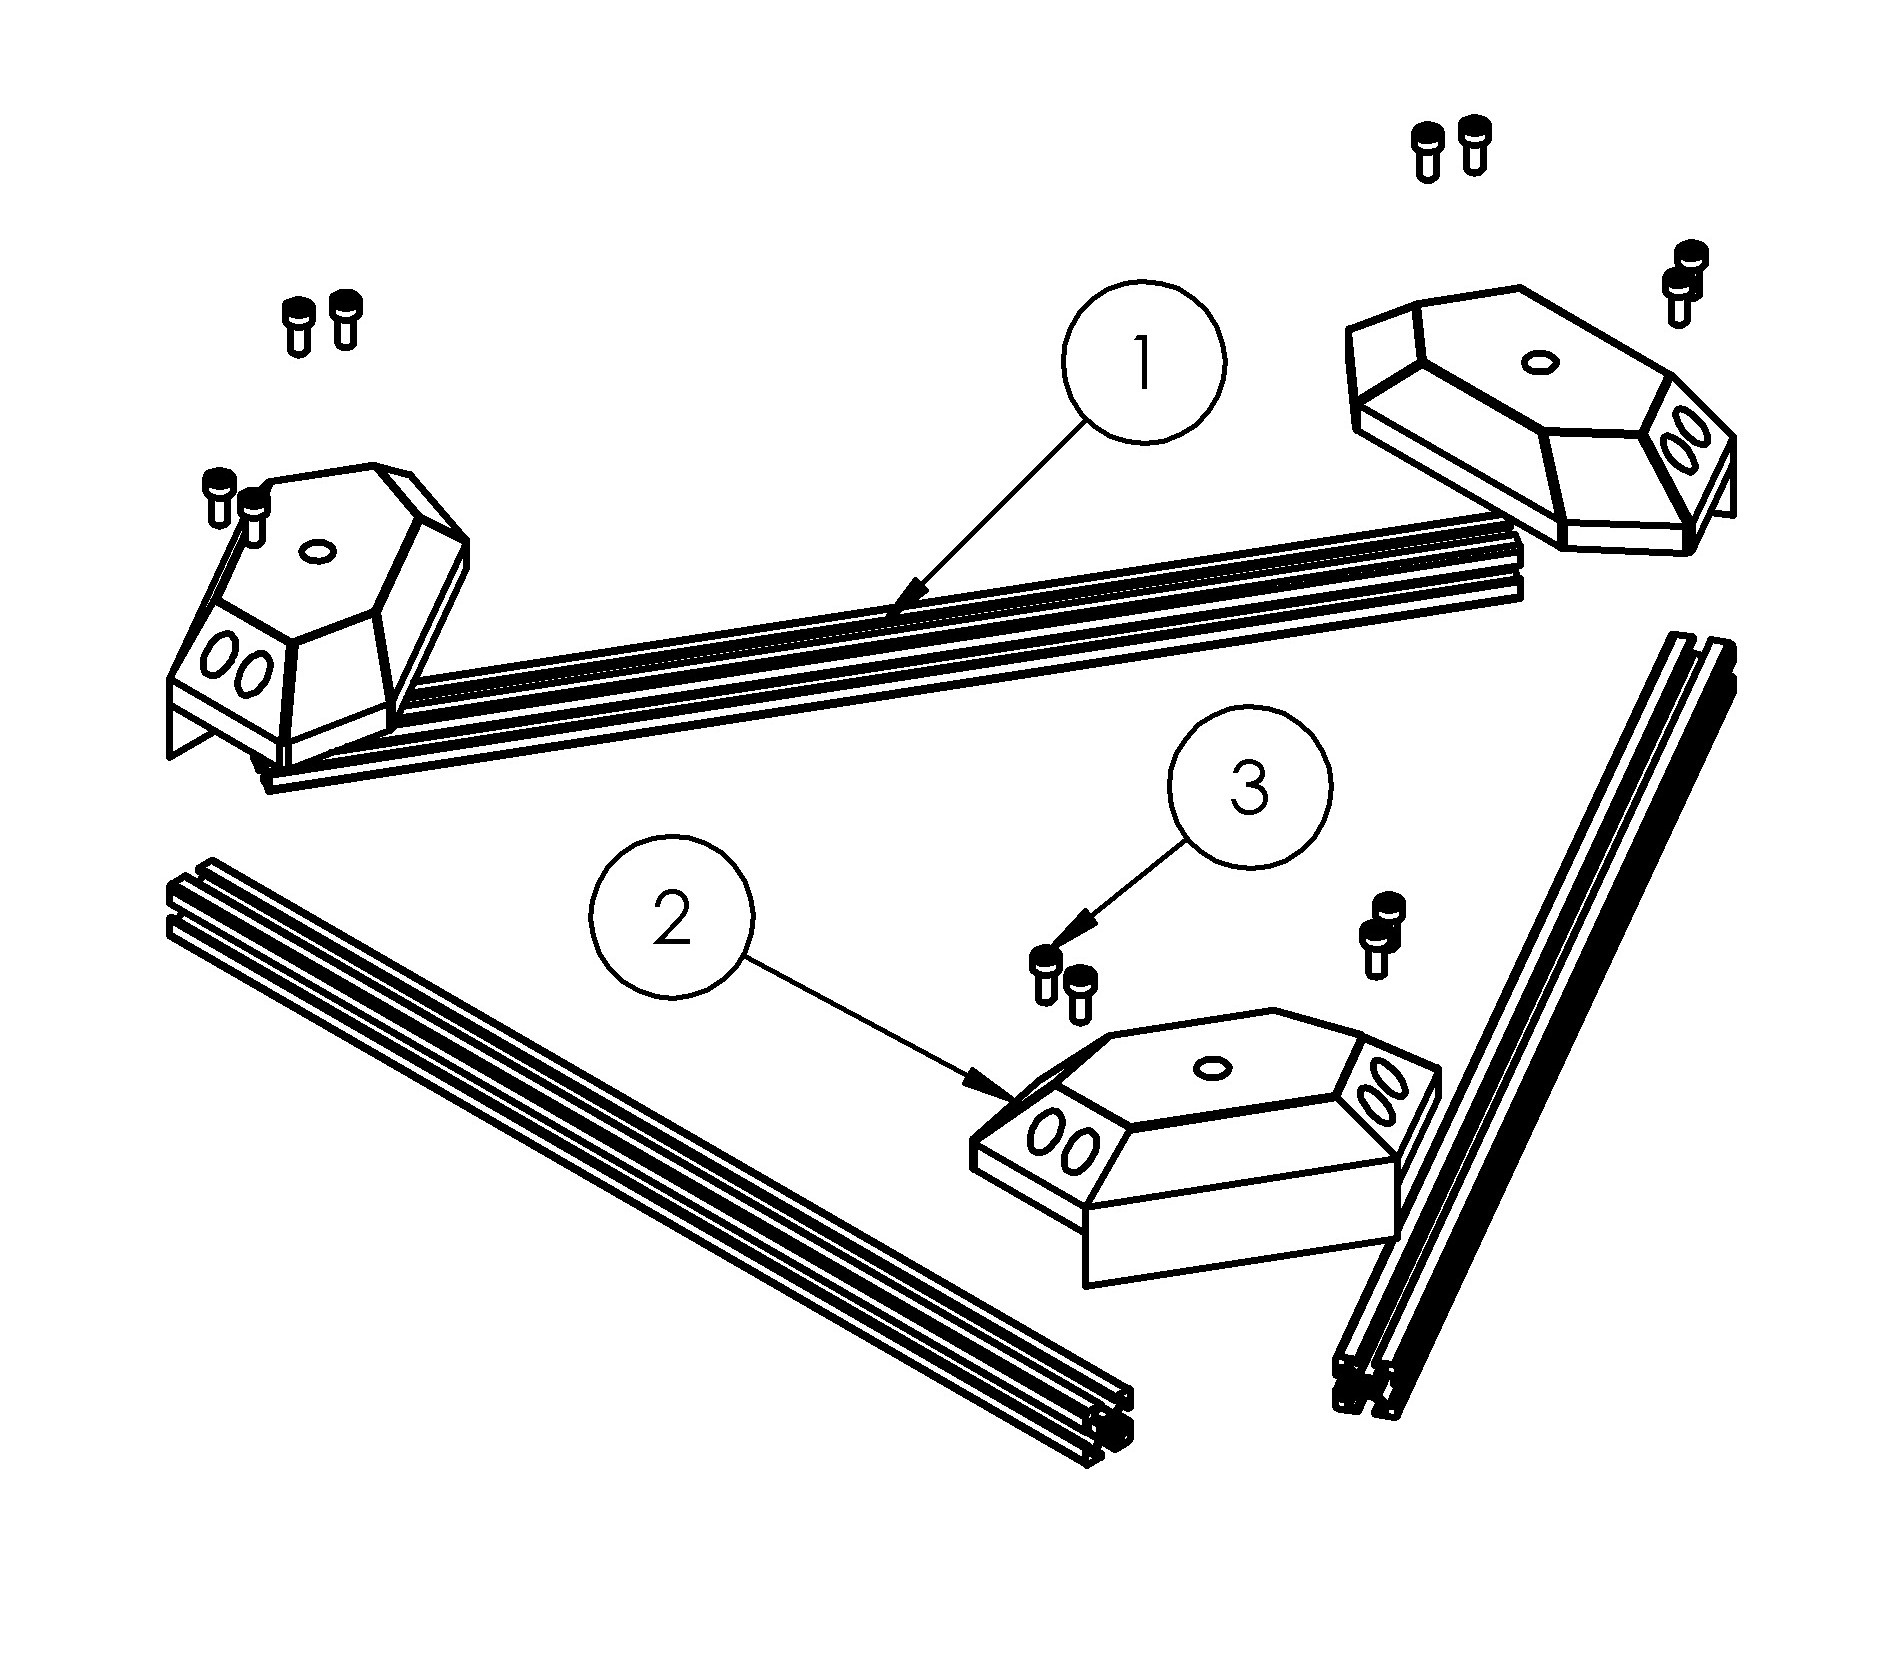
\includegraphics[width=0.70\linewidth]{image/Assem1111.JPG}
    \caption{Base Design of Robot}
    \label{fig:base_design}
\end{figure}

\begin{table}[ht]
    \centering
    \caption{Fixed Base Design Bill of Materials.}
    \label{tab:base_components}
    {\small
    \begin{tabular}{clc}
        \hline
        \textbf{Item} & \textbf{Description} & \textbf{Qty} \\
        \hline
        1 & Aluminium extrusion profile $20 \times 20$\,mm & 3 \\
        2 & 3D-printed PLA corner bracket and motor mount                    & 3 \\
        3 & M4 cap-head bolts and T-nuts  & 12 \\
        \hline
    \end{tabular}}
\end{table}

%--------------------------------------------------------------------
\subsubsection{Bicep Arm Design}
\hspace{1.27cm}
Each upper arm assembly connects one RobStride RS-00 actuator
output shaft to the upper ball-joint end of the corresponding
forearm parallelogram. The exploded view in
\textbf{\autoref{fig:upper_arm}} shows all seven components of
the assembly. The PLA arm body (Item~3) spans $r_f = 200$\,mm
between the motor flange and the forearm joint. On the motor
side, a circular clamping flange (Item~2) with a central
coupling hub (Item~1) is bolted to the arm body using M4
socket-head bolts (Item~5) and secured against the RobStride
RS-00 motor housing via M4 bolts and lock nuts (Item~4). On
the forearm side, the arm terminates in a ball-stud retention
socket that accepts the upper rod-end ball joint of the forearm
parallelogram. The complete assembly is fastened to the motor
output flange using the M4 fastener set (Item~5) distributed
around the bolt circle, with a retaining ring (Item~6) and
the RobStride RS-00 motor body (Item~7, Peak T = 14\,N\,m)
completing the sub-assembly.\par
\hspace{1.27cm}
The PLA arm body was sized to withstand the bending moment
generated by the combined weight and inertia of the forearm
and moving platform during rapid acceleration at the rated
peak torque of 14\,N\,m. The clamping hub ensures a rigid
connection to the motor shaft so that any angular compliance
at this interface, which would manifest as a systematic
position error across the entire workspace, is eliminated.

\begin{figure}[h]
    \centering
    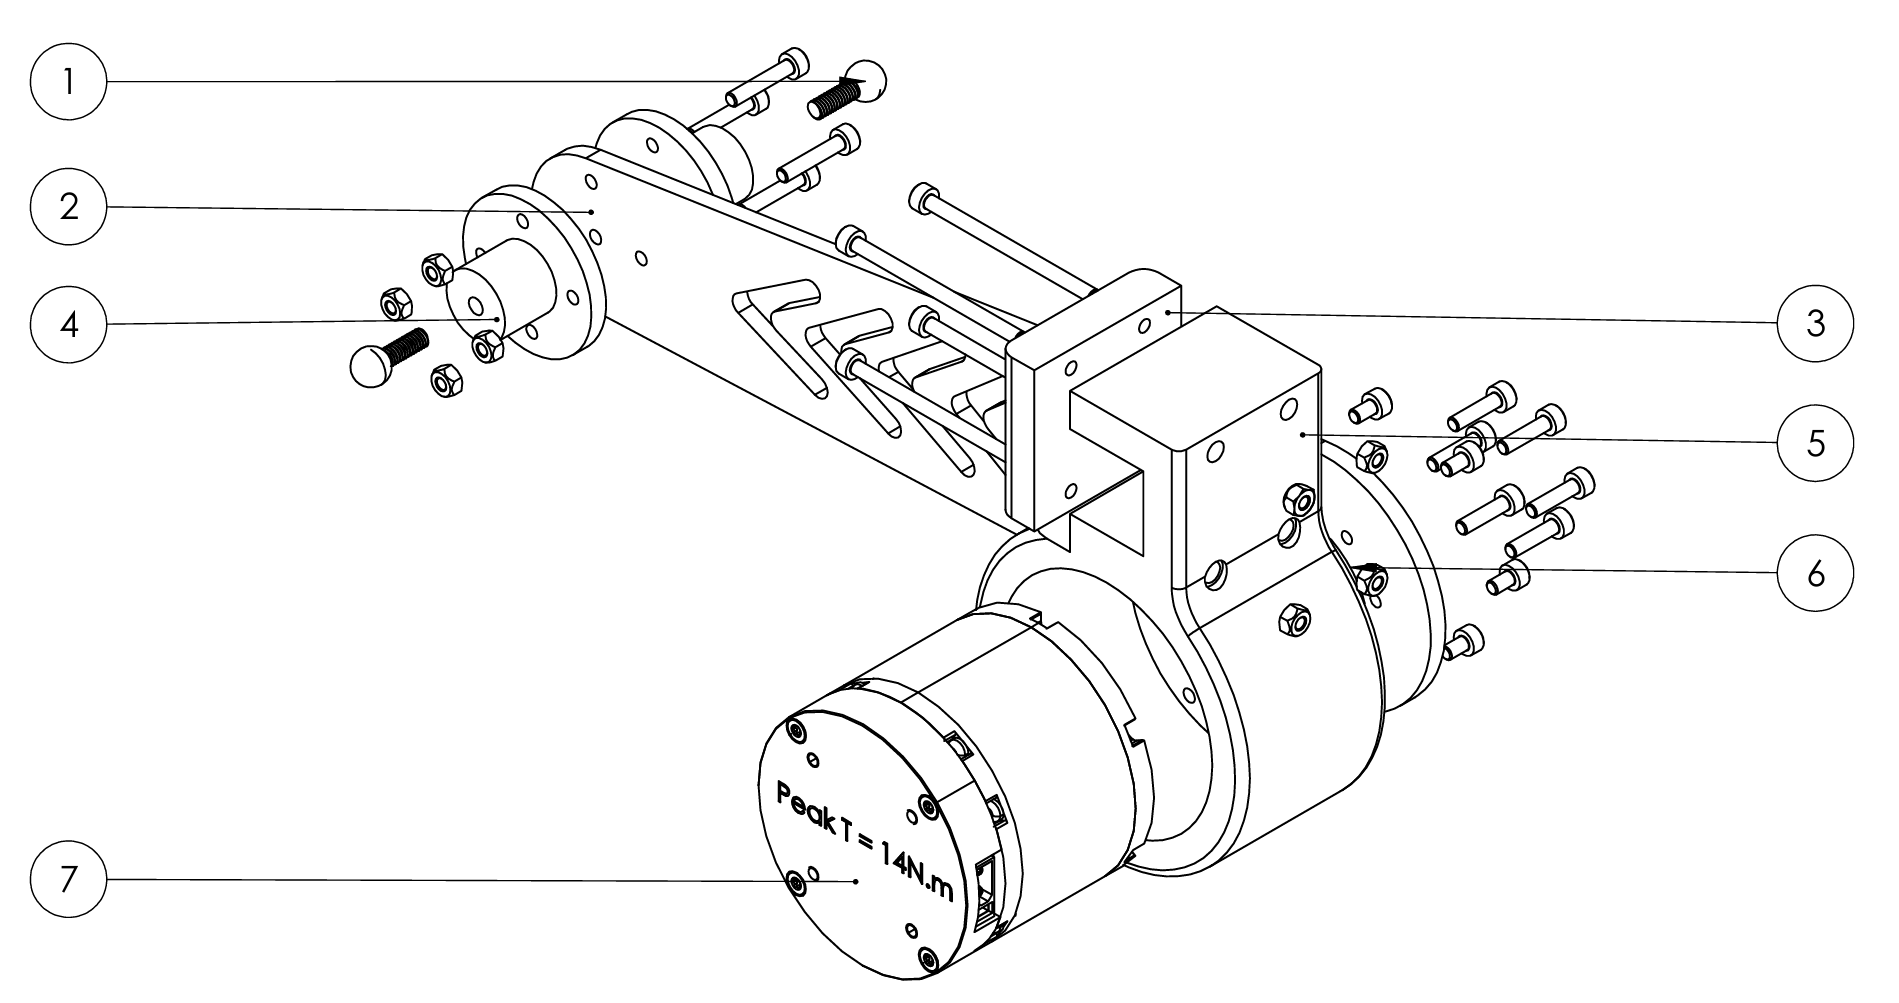
\includegraphics[width=0.85\linewidth]{image/upperarm.png}
    \caption{Bicep Arm of Robot}
    \label{fig:upper_arm}
\end{figure}

\begin{table}[ht]
    \centering
    \caption{Upper Arm Assembly Bill of Materials.}
    \label{tab:upper_arm_components}
    {\small
    \begin{tabular}{clc}
        \hline
        \textbf{Item} & \textbf{Description} & \textbf{Qty} \\
        \hline
        1 & Coupling hub (clamping insert)           & 1 \\
        2 & Circular motor flange plate              & 1 \\
        3 & 3D-printed PLA upper arm body ($r_f = 200$\,mm) & 1 \\
        4 & M4 lock nuts                             & 4 \\
        5 & M4 socket-head cap screws                & 8 \\
        6 & Retaining ring                           & 1 \\
        7 & RobStride RS-00 actuator (Peak T = 14\,N\,m) & 1 \\
        \hline
    \end{tabular}}
\end{table}

%--------------------------------------------------------------------
\subsubsection{Forearm And Moving Platform Design}
\hspace{1.27cm}
The lower arm of each kinematic chain is a parallelogram
linkage connecting the upper arm ball joint to one vertex of
the moving platform. As illustrated in
\textbf{\autoref{fig:lower_arm}}, the assembly consists of
three component types. Item~1 is the carbon fibre forearm rod
of length $r_e = 400$\,mm, terminated at both ends with
aluminium rod-end ball-joint connectors that are press-fitted
and secured with set screws. Two such rods form each
parallelogram pair. Item~2 is the M4 grub screw set used to
lock the rod-end connector to the carbon fibre tube. Item~3 is
the CNC-machined aluminium platform junction plate at the lower
end of the assembly, which provides the bolt pattern for
connecting the forearm ball joints to the moving platform
vertices.\par
\hspace{1.27cm}
The parallelogram geometry is the defining kinematic feature
of the Delta robot: by constraining the two rods to remain
parallel at all configurations, it enforces the condition that
the moving platform undergoes no rotation, maintaining a fixed
end-effector orientation regardless of position within the
workspace \autocite{clavel-1990}. Carbon fibre tube was
selected for the forearm rods because the rods are the only
structural members that undergo full three-dimensional motion
at operating speed. Their mass contributes directly to the
effective inertia seen at the end-effector: reducing rod mass
lowers the torque demand on the actuators during rapid
accelerations and reduces the tendency for the lightweight
parallel linkages to excite structural resonance. The
centre-to-centre spacing between the two rods in each
parallelogram is set equal to the side length $e = 35$\,mm
of the moving platform equilateral triangle, which is the
geometric condition required to maintain the parallelogram
constraint across the full range of joint angles.

\begin{figure}[h]
    \centering
    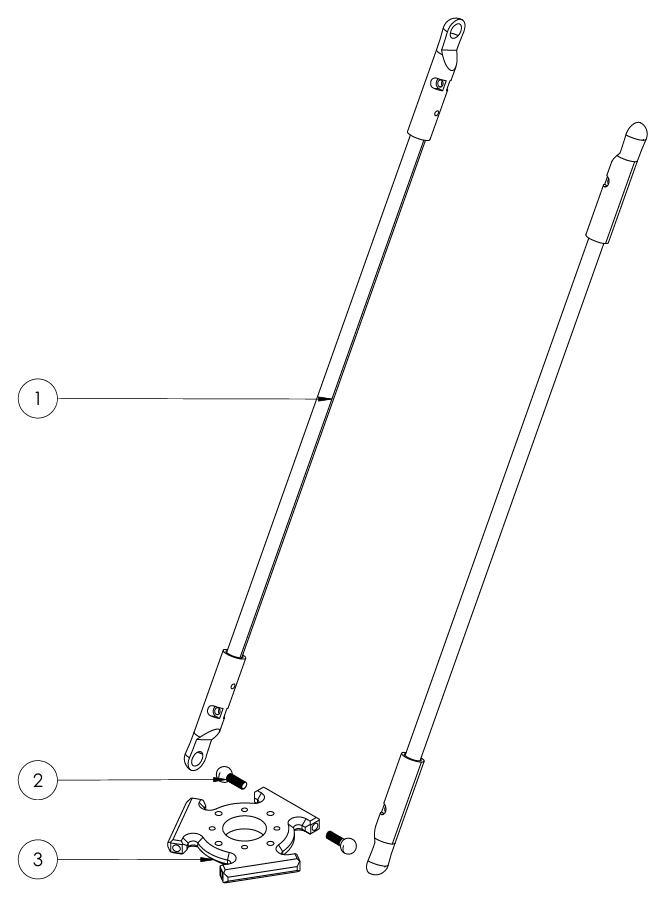
\includegraphics[width=0.55\linewidth]{image/lowerarm.png}
    \caption{Forearm and Moving Plate of Robot}
    \label{fig:lower_arm}
\end{figure}

\begin{table}[ht]
    \centering
    \caption{Lower Arm (Forearm) Assembly Bill of Materials.}
    \label{tab:lower_arm_components}
    {\small
    \begin{tabular}{clc}
        \hline
        \textbf{Item} & \textbf{Description} & \textbf{Qty} \\
        \hline
        1 & Carbon fibre rod with aluminium rod-end
            ball-joint connectors ($r_e = 400$\,mm) & 2 \\
        2 & M4 grub screws (rod-end locking)         & 4 \\
        3 & CNC-machined aluminium platform
            junction plate                           & 1 \\
        \hline
    \end{tabular}}
\end{table}

%--------------------------------------------------------------------
\subsubsection{End-Effector Design}
\hspace{1.27cm}
The end-effector assembly, shown in
\textbf{\autoref{fig:end_effector}}, is a 10-component
sub-assembly mounted below the moving platform. The assembly
integrates a pneumatically actuated two-finger mechanical jaw
gripper, a 650\,nm red-dot laser diode module for end-effector
position tracking, and the structural mounting hardware that
connects the complete assembly to the moving platform centre
boss.\par
\hspace{1.27cm}
Starting from the top of the assembly, Item~1 is the toothed
PLA gripper finger, which has a serrated contact profile to
improve grip on smooth surfaces. Item~2 is the laser diode
module mounting post that positions the 650\,nm beam centrally
between the two jaw fingers and directs it vertically downward
along the end-effector $Z$-axis. Item~3 is the M4 bolt set
used to secure the gripper structure to the cylinder. Item~4
is the M4 finger-to-carrier bolt set fastening the fingers
to the jaw carrier. Item~5 is the CNC-machined aluminium jaw
carrier plate, which transmits the pneumatic cylinder force to
both finger tips simultaneously. Item~6 is the lock-nut set
retaining the assembly. Item~7 is the flat aluminium L-bracket
that mounts the gripper body to the platform junction interface.
Item~8 is the double-acting pneumatic cylinder that actuates
the jaws; pressurised air drives the jaws closed and reversing
the supply opens them. Item~9 is the 3D-printed PLA platform
interface flange that bolts the complete end-effector to the
central boss of the moving platform. Item~10 is the M4 bolt
set securing the flange to the platform.\par
\hspace{1.27cm}
The solenoid valve controlling the pneumatic cylinder is
commanded via CAN ID\,4, with \texttt{004\#01} to close and
\texttt{004\#00} to open. The 5\,mW, 650\,nm laser module
operates continuously during pick-and-place trials and
provides the fiducial dot used by the visual end-effector
feedforward correction loop: the camera detects the laser dot
projected onto the belt surface, computes the pixel offset
between the dot centroid and the target object centroid, and
issues iterative correction commands until alignment converges
before the gripper descends to the pick depth.\par
\hspace{1.27cm}
The vertical distance from the moving platform centre to the
jaw finger contact face defines the end-effector offset
$\delta z$, which is added to the platform $z$-coordinate in
the IK solver when computing the joint angles required to
position the gripper tips at the belt surface. This offset
was measured from the fabricated assembly and is listed in
\autoref{tab:mechanical_params}.

\begin{figure}[h]
    \centering
    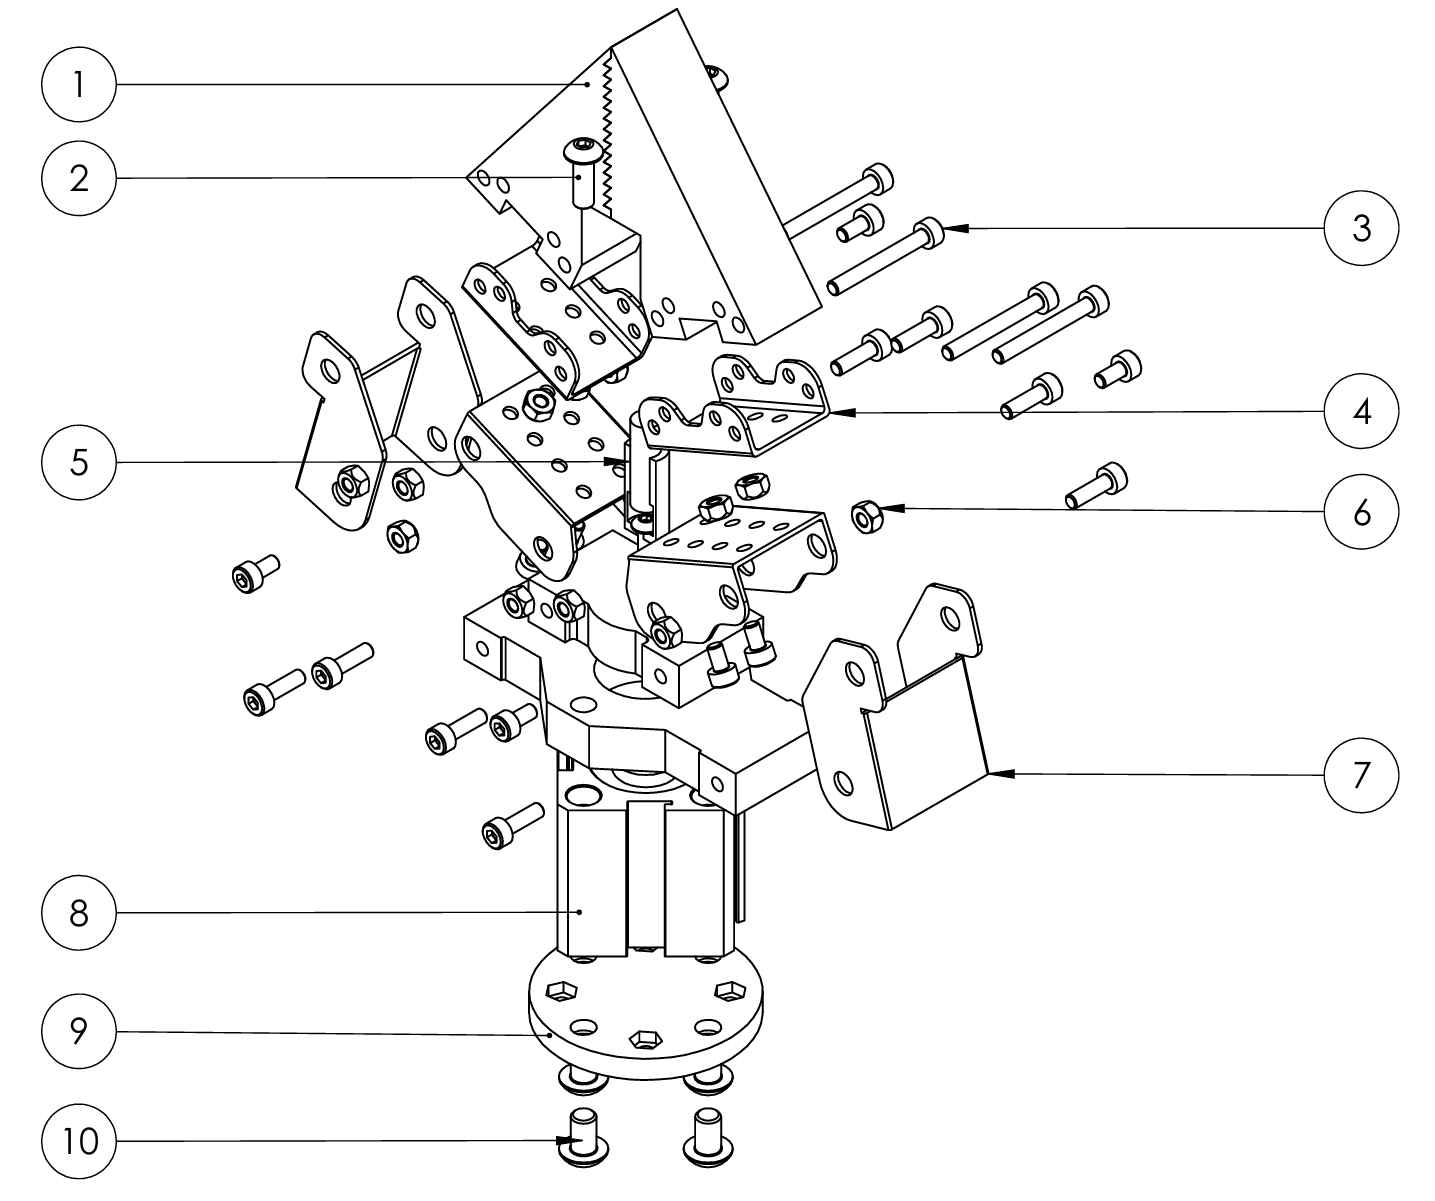
\includegraphics[width=0.75\linewidth]{image/end_effector.png}
    \caption{End-Effector of Robot}
    \label{fig:end_effector}
\end{figure}

\begin{table}[ht]
    \centering
    \caption{End-Effector Assembly Bill of Materials.}
    \label{tab:end_effector_components}
    {\small
    \begin{tabular}{clc}
        \hline
        \textbf{Item} & \textbf{Description} & \textbf{Qty} \\
        \hline
        1  & 3D-printed PLA toothed gripper finger         & 2 \\
        2  & Laser diode module mounting post (650\,nm, 5\,mW)     & 1 \\
        3  & M4 gripper structure-to-cylinder bolt set             & 2 \\
        4  & M4 finger-to-carrier bolt set                         & 4 \\
        5  & CNC aluminium jaw carrier plate                       & 1 \\
        6  & Lock nuts                                             & 12 \\
        7  & Aluminium L-bracket (gripper-to-platform)             & 2 \\
        8  & Double-acting pneumatic cylinder                      & 1 \\
        9  & 3D-printed PLA platform interface flange              & 1 \\
        10 & M4 flange-to-platform bolt set                        & 4 \\
        \hline
    \end{tabular}}
\end{table}

%--------------------------------------------------------------------
\subsubsection{Design Parameters Summary}
\hspace{1.27cm}
The complete mechanical parameters of the fabricated Delta robot
prototype are summarised in \autoref{tab:mechanical_params}.
These values were used directly as inputs to the analytical IK
and FK solvers described in \autoref{sec:kinematics}.

\begin{table}[h]
    \centering
    \caption{Delta Robot Mechanical Design Parameters.}
    \label{tab:mechanical_params}
    \begin{tabular}{llcc}
        \hline
        \textbf{Parameter} & \textbf{Symbol} &
        \textbf{Value} & \textbf{Unit} \\
        \hline
        Base triangle side length   & $f$
            & 157     & mm \\
        Platform triangle side      & $e$
            & 35      & mm \\
        Upper arm length            & $r_f$
            & 200     & mm \\
        Forearm length              & $r_e$
            & 400     & mm \\
        Nominal pick depth (platform) & $Z_{\text{pick}}$
            & $-500$  & mm \\
        Target workspace radius     & $r_w$
            & 150     & mm \\
        End-effector offset         & $\delta z$
            & 150     & mm \\
        Actuator peak torque        & $T_{\text{peak}}$
            & 14      & N\,m \\
        \hline
        Base frame material         & --
            & \multicolumn{2}{c}{Aluminium extrusion
              $20 \times 20$\,mm} \\
        Upper arm material          & --
            & \multicolumn{2}{c}{3D-printed PLA} \\
        Forearm rod material        & --
            & \multicolumn{2}{c}{Carbon fibre tube} \\
        Moving platform material    & --
            & \multicolumn{2}{c}{CNC aluminium} \\
        Gripper body material       & --
            & \multicolumn{2}{c}{CNC aluminium} \\
        Finger material             & --
            & \multicolumn{2}{c}{3D-printed PLA (toothed)} \\
        Gripper actuation           & --
            & \multicolumn{2}{c}{Pneumatic (double-acting)} \\
        EE laser                    & --
            & \multicolumn{2}{c}{650\,nm, 5\,mW red-dot diode} \\
        Gripper CAN ID              & --
            & \multicolumn{2}{c}{ID\,4
              (\texttt{004\#01} / \texttt{004\#00})} \\
        \hline
    \end{tabular}
\end{table}

%============================================================================
% END OF MECHANICAL DESIGN SECTION
%============================================================================

\subsection{Hardware Selection}
\subsubsection{Motors}
\hspace{1.27cm}
The RobStride RS-00 is a compact quasi-direct-drive (QDD)
actuator integrating a brushless DC motor, a low-ratio
planetary gearbox, and an absolute magnetic encoder in a
single module. QDD actuators offer high backdrivability,
low reflected inertia, and high-bandwidth torque control
compared to conventional high-ratio gearbox motors, making
them well suited for compliant robotic manipulation. Three
RS-00 units (CAN IDs 1, 2, and 3) are used, one per
kinematic chain, mounted on the fixed base frame.

\begin{figure}[h]
    \centering
    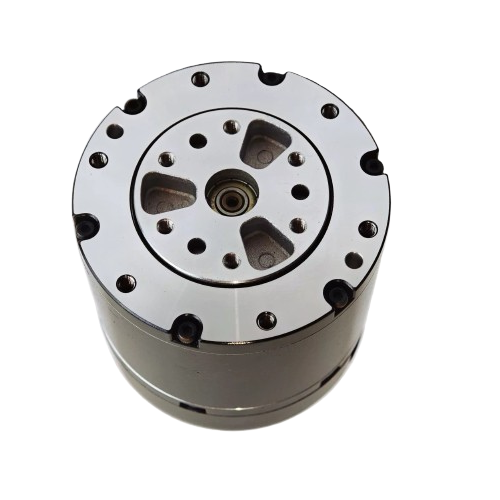
\includegraphics[width=0.4\linewidth]{image/ROBSTRIDE-00.png}
    \caption{RobStride RS-00 quasi-direct-drive actuator.}
    \label{fig:motor}
\end{figure}

\begin{table}[htbp]
    \centering
    \caption{RobStride RS-00 Specifications.}
    \label{tab:motor_spec}
    {\small
    \begin{tabular}{lcc}
        \hline
        \textbf{Parameter} & \textbf{Value} & \textbf{Unit} \\
        \hline
        Rated voltage           & 24      & V \\
        Peak torque             & 14.0    & N\,m \\
        Max motor speed         & 50.0    & rad/s \\
        Max motor acceleration  & 100.0   & rad/s$^2$ \\
        Medium preset velocity  & 25.0    & rad/s \\
        Medium preset accel.    & 50.0    & rad/s$^2$ \\
        Communication           & CAN bus & -- \\
        CAN baudrate            & 1       & Mbit/s \\
        Encoder type            & Absolute magnetic & -- \\
        Control mode            & Position-Profile (PP) & -- \\
        \hline
    \end{tabular}}
\end{table}

\hspace{1.27cm}
In this system the RS-00 is operated exclusively in
\textbf{Position-Profile (PP) mode}, whose internal
control architecture is illustrated in
\textbf{\autoref{fig:pp_mode}}. PP mode executes a
complete closed-loop trajectory internally within the
motor controller. The host PC supplies three set-points
per move: target angle, set speed, and set acceleration.
The onboard \textbf{t-curve planning algorithm} generates
a time-optimal trapezoidal velocity profile from these
set-points and outputs a continuously updated planning
perspective (the instantaneous position reference).\par
\hspace{1.27cm}
The planning perspective is compared with the current
encoder angle to form a position error. This error is
amplified by the proportional gain $K_p$ of the position
loop, whose output becomes the velocity reference. A
second subtraction node compares this reference against
the current speed measured by the encoder to produce a
velocity error, which feeds a \textbf{PI velocity
controller}. The PI output is a torque (current) demand
that passes through a \textbf{torque protection} saturation
block, limiting the command to the rated peak current to
prevent thermal damage.\par
\hspace{1.27cm}
The protected torque demand is decomposed into two current
references following field-oriented control (FOC)
conventions: the quadrature-axis reference
$i_{q,\text{ref}}$ (torque-producing component) is set to
the torque demand value, while the direct-axis reference
$i_{d,\text{ref}} = 0$ (flux component) is held at zero
for maximum torque-per-ampere efficiency. Two independent
\textbf{PI current controllers} regulate $i_q$ and $i_d$
respectively, producing voltage references that are
modulated by a \textbf{Space Vector PWM (SVPWM)} block.
The SVPWM signals drive the \textbf{three-phase voltage
inverter}, which applies the commanded phase voltages to
the brushless DC motor windings to produce the desired
torque and motion.

\begin{figure}[h]
    \centering
    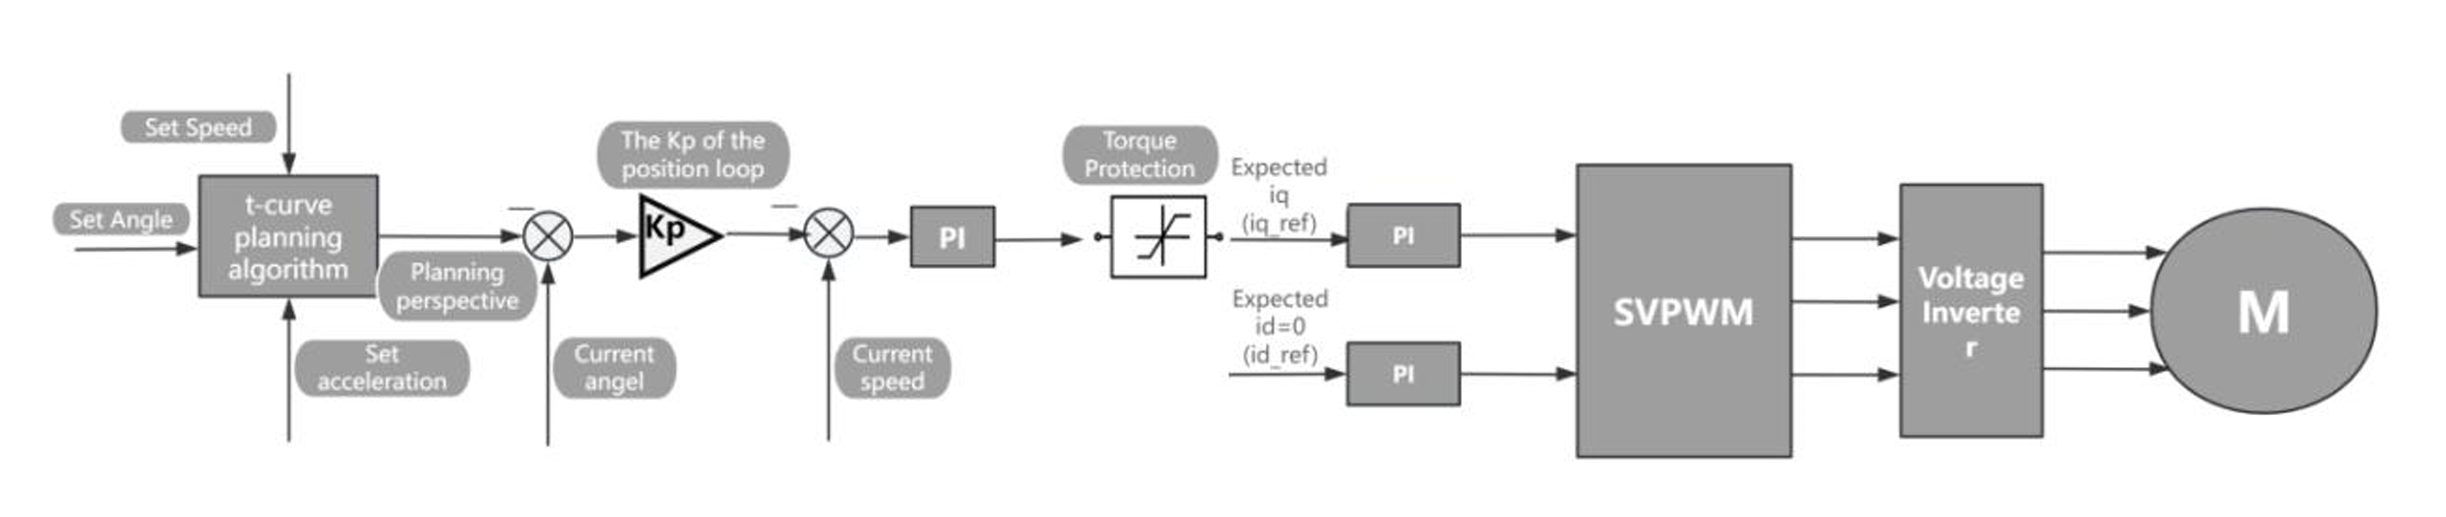
\includegraphics[width=0.95\linewidth]{image/PPmode.png}
    \caption{Position-Profile (PP) Mode Control Architecture
             of The RobStride RS-00 Actuator.}
    \label{fig:pp_mode}
\end{figure}
\subsubsection{Motor Bridge}
\begin{itemize}
    \par
    \hspace{1.27cm}
    The RobStride RS-00 motors are driven directly over a CAN bus at 1\,Mbit/s using a USB-to-CAN adapter connected to the host PC running Ubuntu 22.04 with ROS\,2 Humble. The SocketCAN Linux kernel driver exposes the CAN interface as a standard network interface (\texttt{can0}), enabling direct read/write access from Python via the \texttt{python-can} library. The three motor driver boards are connected in a daisy-chain topology on the same CAN bus, with termination resistors at both ends.
    \par
    \begin{figure}[h]
        \centering
         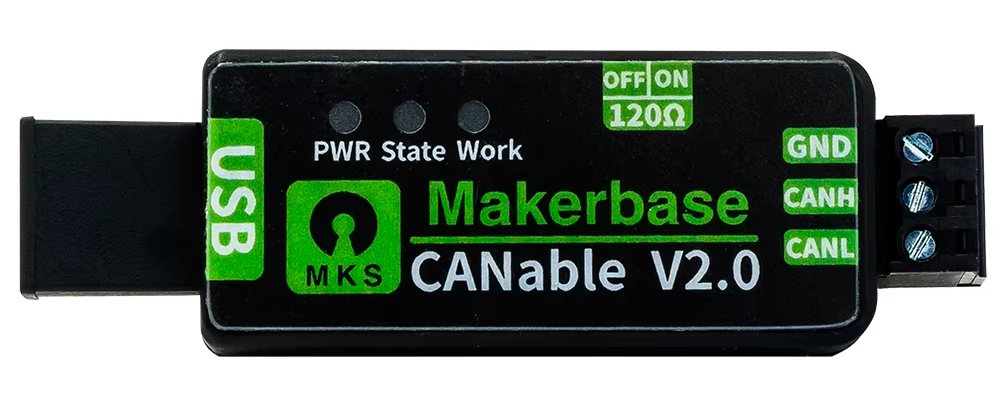
\includegraphics[width=0.4\linewidth]{image/can driver.png}
        \caption{USB-to-CAN Adapter for ROS\,2 CAN Bus Interface.}
        \label{fig:driver}
    \end{figure}
    \begin{table}[htbp]
        \centering
        \caption{CAN Bus Interface Specifications.}
        {\small
        \begin{tabular}{lcc}
            \textbf{Parameter} & \textbf{Specification} & \textbf{Unit} \\
            \hline
            Interface type    & USB-to-CAN      & — \\
            Linux driver      & SocketCAN       & — \\
            Baudrate          & 1               & Mbit/s \\
            Topology          & Daisy-chain     & — \\
            Motor nodes       & 3 (IDs 1, 2, 3) & — \\
            Gripper node      & 1 (ID 4)        & — \\
            Host OS           & Ubuntu 22.04    & — \\
            \ChangeRT{1.5pt}
        \end{tabular}}
        \label{tab:driver_spec}
    \end{table}
\end{itemize}
\subsubsection{Pneumatic Solenoid Valve}
\hspace{1.27cm}
The pneumatic solenoid valve used in this system is a
five-port, two-position (5/2) single-solenoid directional
control valve, as shown in \textbf{\autoref{fig:pneumatic_valve}}.
The valve body is constructed from anodised aluminium alloy
with an IP65-rated solenoid coil housing, rated for continuous
duty (100\,\% ED) at DC\,24\,V, drawing 200\,mA at a power
consumption of 4.8\,W. The operating voltage range is
DC\,20.4\,V to 28.4\,V, making it directly compatible with
the 24\,V power rail of the system.

\par
\hspace{1.27cm}
The valve has three external connections visible in
\textbf{\autoref{fig:pneumatic_valve}}: a single \textbf{Air
Inlet Hole} on the underside that receives compressed air from
the air container, and two \textbf{Air Outlet Holes} (port~A
and port~B) on the upper face that route air to the two
chambers of the double-acting pneumatic cylinder on the
gripper assembly. When the solenoid coil is de-energised, the
internal spring returns the spool to its default position,
directing compressed air from the inlet to outlet port~A and
venting port~B to atmosphere, which drives the gripper jaws to
the open position. When the solenoid coil is energised by the
CAN ID\,4 command \texttt{004\#01}, the magnetic force shifts
the spool to connect the inlet to port~B and vent port~A,
driving the jaws to the closed (grip) position. Sending
\texttt{004\#00} de-energises the coil and returns the valve
to the open state.\par
\hspace{1.27cm}
The 5/2 configuration was selected because the double-acting
pneumatic cylinder on the end-effector requires independent
pressurisation of both its extend and retract chambers to
produce positive gripping force in both the closing and
opening directions, rather than relying on a return spring.
This provides faster jaw opening response and more consistent
release behaviour than a spring-return cylinder, which is
important for repeatable object placement at the drop position
during pick-and-place cycles. The IP65 ingress protection
rating ensures reliable operation in the laboratory environment
where compressed air fittings may introduce moisture.

\begin{figure}[h]
    \centering
    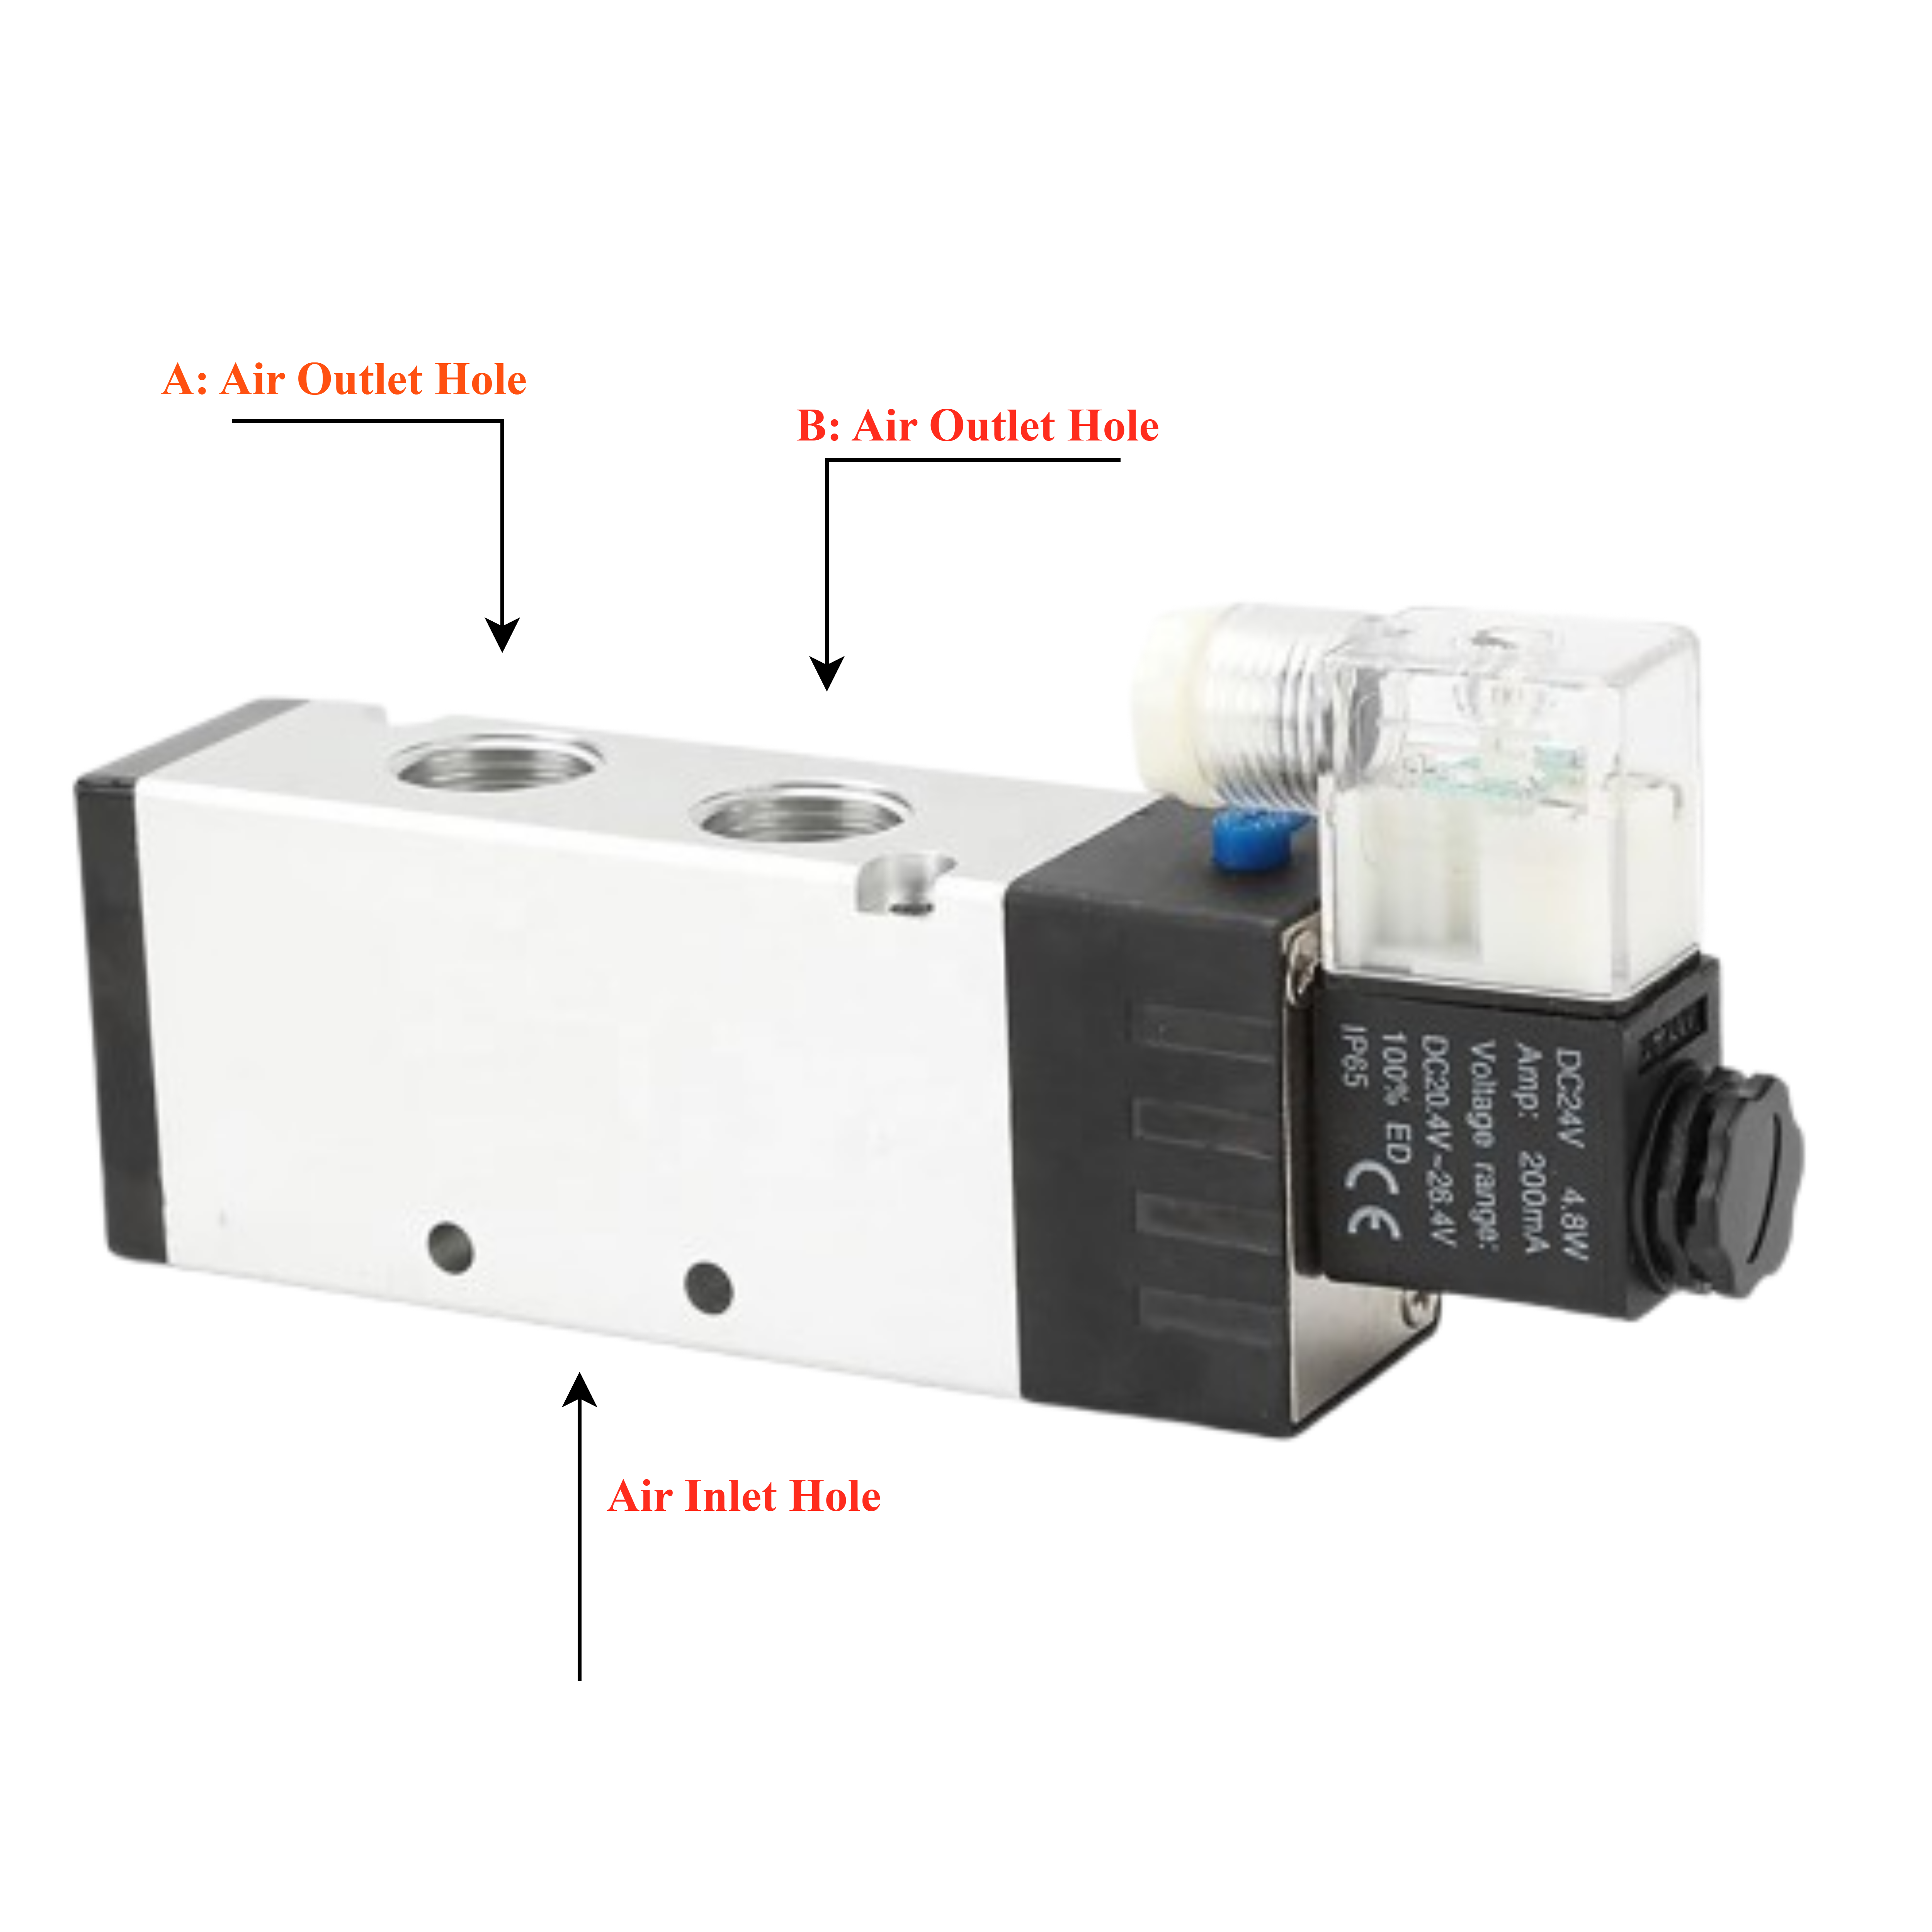
\includegraphics[width=0.60\linewidth]{image/Pneumatic.png}
    \caption{5/2 single-solenoid directional control valve
             (DC\,24\,V, 4.8\,W, 200\,mA, IP65) showing the
             air inlet hole on the underside and the two air
             outlet holes (port~A and port~B) on the upper
             face that supply the double-acting gripper
             cylinder.}
    \label{fig:pneumatic_valve}
\end{figure}

\begin{table}[htbp]
    \centering
    \caption{Pneumatic Solenoid Valve Specifications.}
    \label{tab:pneumatic_spec}
    {\small
    \begin{tabular}{lcc}
        \hline
        \textbf{Parameter} & \textbf{Value} & \textbf{Unit} \\
        \hline
        Valve type              & 5/2 single-solenoid & -- \\
        Solenoid voltage        & DC 24       & V \\
        Voltage range           & DC 20.4--28.4 & V \\
        Power consumption       & 4.8         & W \\
        Solenoid current        & 200         & mA \\
        Duty cycle              & 100 (continuous) & \% ED \\
        Ingress protection      & IP65        & -- \\
        Air inlet               & 1 port (underside) & -- \\
        Air outlets             & 2 ports A, B (top) & -- \\
        Control interface       & CAN ID\,4   & -- \\
        Close command           & \texttt{004\#01} & -- \\
        Open command            & \texttt{004\#00} & -- \\
        \hline
    \end{tabular}}
\end{table} 
\subsubsection{Camera and Vision Hardware}
\hspace{1.27cm}
The Intel RealSense D455 is a stereo-capable RGB-D camera selected for this system due to its wide field of view, stable USB\,3.0 interface, and well-supported ROS\,2 driver. In this application, only the RGB stream is used for object detection and localisation. Since all pick targets lie on the conveyor belt surface at a fixed and known elevation of $Z = -410$\,mm below the robot base frame, per-pixel depth sensing is not required. Object positions are recovered from 2D pixel coordinates using the known camera intrinsics and the fixed belt depth, as described in the vision pipeline section. The camera connects to the host PC via USB\,3.0 and is driven by the \texttt{librealsense2} driver and \texttt{realsense2\_camera} ROS\,2 wrapper node.

\par
    \begin{figure}[h]
        \centering
         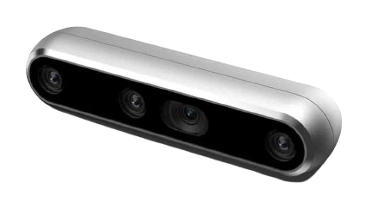
\includegraphics[width=0.4\linewidth]{image/Realsense D455.png}
        \caption{The Intel RealSense D455.}
        \label{fig:Realsense D455}
    \end{figure}

\begin{table}[htbp]
    \centering
    \caption{Intel RealSense D455 Specifications.}
    {\small
    \begin{tabular}{lcc}
        \textbf{Parameter} & \textbf{Specification} & \textbf{Unit} \\
        \hline
        Depth technology     & Active IR stereo   & — \\
        Stereo baseline      & 95                 & mm \\
        RGB resolution       & $640 \times 480$   & px \\
        Depth resolution     & $848 \times 480$   & px \\
        Frame rate           & 30                 & fps \\
        Depth range          & 0.4 -- 6.0         & m \\
        RGB FOV (H$\times$V) & 87$\times$58       & deg \\
        Interface            & USB 3.0            & — \\
        \ChangeRT{1.5pt}
    \end{tabular}}
    \label{tab:camera_spec}
\end{table}

\subsubsection{Output2CAN}
\hspace{1.27cm}
The Output2CAN board is a custom CAN-based controller developed by the Cambodia Team and used in many projects specifically to control pneumatic actuators. In the Delta robot system, this board is responsible for managing the vacuum gripper through solenoid valve control. At its core, the board is powered by an STM32F103C8T6 microcontroller, which receives CAN messages from the main controller and triggers digital outputs accordingly. These outputs are connected to N-MOSFET drivers capable of switching standard 12V solenoid valves on and off. Four output channels are available (D1–D4). Communication with the robot’s CAN network is handled via an onboard TJA1050 transceiver, which ensures robust and noise-resistant signaling. The board features clearly labeled JST connectors for each output, simplifying cable management and allowing for quick installation and maintenance. Power is supplied via separate VCC and GND lines, while the logic section is powered by a regulated 3.3V supply.\par
\begin{figure}[h]
    \centering  
    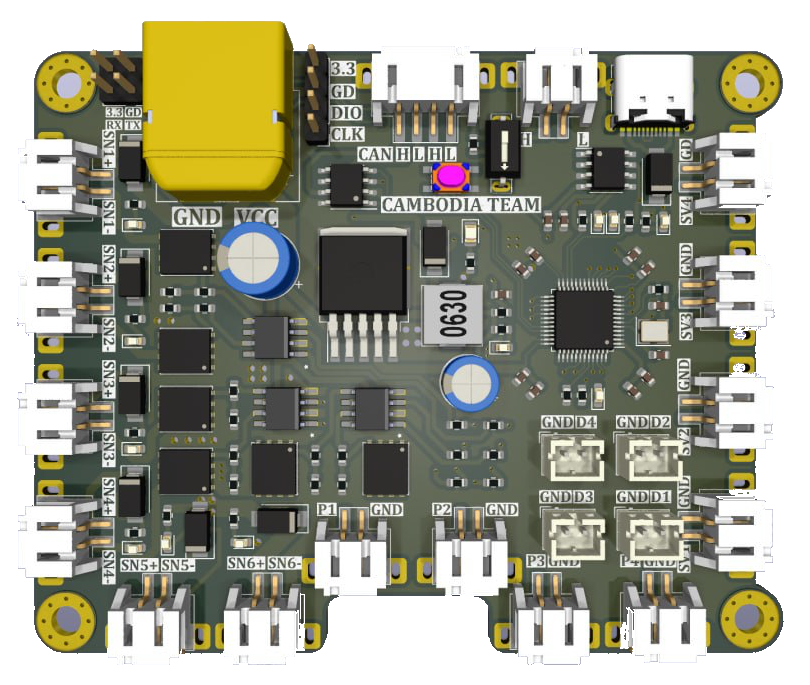
\includegraphics[width=0.5\linewidth]{image/output2can.png}
    \caption{Output2CAN board.}
    \label{fig:output2can}
\end{figure}
\hspace{1.27cm}
By delegating pneumatic control to this dedicated module, the overall wiring complexity is reduced and the system becomes more modular and maintainable. This makes the Output2CAN board an efficient solution for decentralized pneumatic actuation within the Delta robot platform.

\subsubsection{Conveyor Belt Hardware}
\hspace{1.27cm}
The conveyor belt is driven by a NEMA-17 stepper motor through a 1:36 planetary gearbox, with a timing pulley of circumference 153.9\,mm ($\pi \times 49$\,mm). The stepper motor is controlled by an Arduino microcontroller running at 1/8 microstepping (1600 steps/revolution) with a step pulse delay of 104\,\textmu s, yielding a physically measured belt speed of 12.85\,mm/s in the $Y$ direction (toward the EXIT side of the workspace).
\par
    \begin{figure}[h]
        \centering
         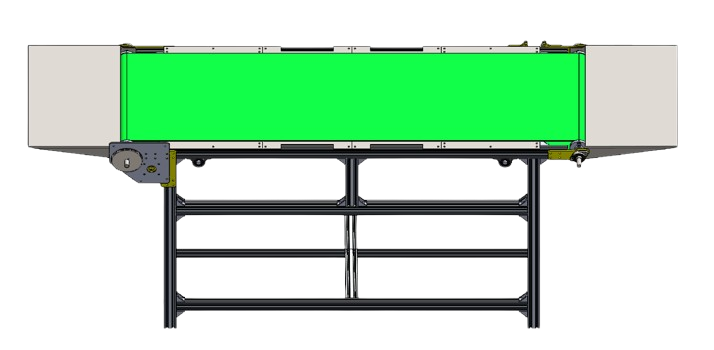
\includegraphics[width=0.7\linewidth]{image/Conveyer.png}
        \caption{Conveyer Belt.}
        \label{fig:Conveyer}
    \end{figure}

%============================================================================
\subsection{Kinematic Model Development}
\hspace{1.27cm}
The kinematic model of the Delta robot establishes the mathematical relationship between joint space (motor angles $\theta_1, \theta_2, \theta_3$) and Cartesian task space (end-effector position $x, y, z$). Both forward and inverse kinematics are derived based on the geometric parameters of the robot following the formulation of \autocite{clavel-1990} as implemented by \autocite{mzavatsky-2009}.

\subsubsection{Geometric Parameters}
\hspace{1.27cm}
The Delta robot is characterised by four geometric parameters listed in \textbf{\autoref{tab:delta_params}}. The fixed base equilateral triangle has a side
length of $f = 157$ mm, and the moving platform equilateral triangle has a side
length of $e = 35$ mm. The upper arm length is $r_f = 200$ mm, and the lower arm
(forearm) length is $r_e = 400$ mm. The reference coordinate frame is placed at
the center of symmetry of the fixed base triangle, with the $z$-axis pointing
downward such that all reachable end-effector positions carry negative
$z$-coordinates. \par
\begin{table}[htbp]
    \centering
    \caption{Delta Robot Geometric Parameters.}
    {\small
    \begin{tabular}{clcc}
        \textbf{Symbol} & \textbf{Description} & \textbf{Value} & \textbf{Unit} \\
        \hline
        $f$   & Side length of fixed base triangle   & 157 & mm \\
        $e$   & Side length of moving platform        & 35  & mm \\
        $r_f$ & Upper arm length                      & 200 & mm \\
        $r_e$ & Lower arm (forearm) length             & 400 & mm \\
        \ChangeRT{1.5pt}
    \end{tabular}}
    \label{tab:delta_params}
\end{table}
To simplify the kinematic equations, the effective radius difference is defined as:
\begin{equation}
    \Delta r = \frac{f}{2\sqrt{3}} - \frac{e}{2\sqrt{3}}
             = \frac{157}{2\sqrt{3}} - \frac{35}{2\sqrt{3}}
             \approx 45.34 - 10.10
             = 35.24 \text{ mm}
    \label{eq:delta_r}
\end{equation}
This quantity $\Delta r$ represents the horizontal offset between the base joint
pivot and the effective platform attachment point for each arm, and appears
directly in the inverse kinematics equations.
\par
\begin{figure}[h]
    \centering
    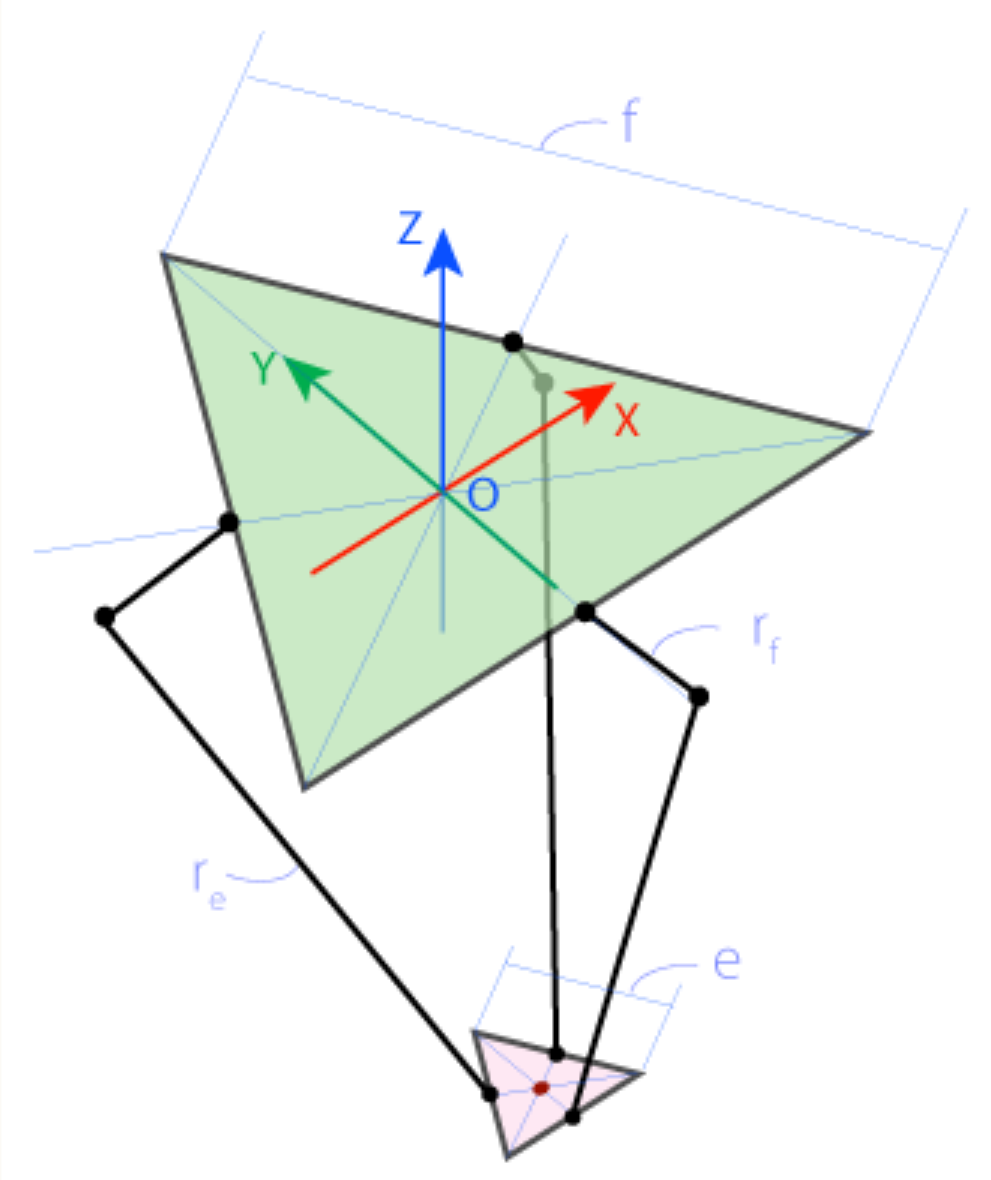
\includegraphics[width=0.6\linewidth]{image/Schem Kinematic.png}
    \caption{Delta Robot Kinematic Scheme ($f=157$\,mm, $e=35$\,mm, $r_f=200$\,mm, $r_e=400$\,mm).}
    \label{fig:kinematic_scheme}
\end{figure}

\subsubsection{Inverse Kinematics}
\hspace{1.27cm}
The inverse kinematics (IK) determines the three joint angles $(\theta_1, \theta_2, \theta_3)$
required to position the end-effector at a desired Cartesian coordinate $(x_0, y_0, z_0)$.
Due to the three-fold rotational symmetry of the Delta robot, each arm is solved independently
after rotating the target coordinates by $0°$, $120°$, and $240°$ respectively about the $z$-axis.

\par\noindent\textbf{Step 1: Coordinate Rotation}\par
\hspace{1.27cm}
For arm $i$ ($i = 1, 2, 3$), the end-effector target point is first rotated into the reference
plane of that arm. Defining the rotation angle $\varphi_i = (i - 1) \times 120°$, the rotated
coordinates are:

\begin{equation}
    x'_i = x_0 \cos\varphi_i + y_0 \sin\varphi_i
    \label{eq:rot_x}
\end{equation}
\begin{equation}
    y'_i = -x_0 \sin\varphi_i + y_0 \cos\varphi_i
    \label{eq:rot_y}
\end{equation}
\begin{equation}
    z'_i = z_0
    \label{eq:rot_z}
\end{equation}

This rotation reduces the 3D problem for each arm to an equivalent planar problem
in the $YZ$ plane of that arm's reference frame.

\par\noindent\textbf{Step 2: Effective Target Point}\par
\hspace{1.27cm}
The effective target point for each arm accounts for the geometric offset $\Delta r$
between the base pivot and the platform joint:

\begin{equation}
    y_{i,\text{eff}} = y'_i - \Delta r = y'_i - 35.24 \text{ mm}
    \label{eq:eff_target}
\end{equation}
\hspace{1.27cm}
The joint angle $\theta_i$ for arm $i$ is then found by solving the intersection of two
circles in the $YZ$ plane: a circle of radius $r_f = 200$ mm centred at the base pivot
$F_i$, and a circle of radius $r_e = 400$ mm centred at the effective target point.

\par\noindent\textbf{Step 3: Planar Circle Intersection}\par
\hspace{1.27cm}
Expanding the two circle equations and subtracting to eliminate the quadratic terms
yields a linear expression. Substituting back gives the following quadratic in $y_J$:
\begin{equation}
    a \cdot y_J^2 + b \cdot y_J + c = 0
    \label{eq:quadratic}
\end{equation}

where:

\begin{equation}
    a = 1 + \left(\frac{z'_i}{y_{i,\text{eff}}}\right)^2
    \label{eq:coeff_a}
\end{equation}

\begin{equation}
    b = \frac{-2 \, y_{i,\text{eff}} \left(r_e^2 - r_f^2 - y_{i,\text{eff}}^2 - z_i^{\prime 2}\right)}
            {2\, y_{i,\text{eff}}^2 + 2\, z_i^{\prime 2}}
    \label{eq:coeff_b}
\end{equation}

\begin{equation}
    c = \left(\frac{r_e^2 - r_f^2 - y_{i,\text{eff}}^2 - z_i^{\prime 2}}
                   {2\, y_{i,\text{eff}}}\right)^2 - r_f^2
    \label{eq:coeff_c}
\end{equation}
\hspace{1.27cm}
The discriminant $D = b^2 - 4ac$ must be non-negative for a valid solution. A negative
discriminant indicates that the target position lies outside the reachable workspace, and
the IK solver immediately rejects the command and returns an error flag before any motor
command is issued.

\par\noindent\textbf{Step 4: Joint Angle Recovery}\par
\hspace{1.27cm}
Selecting the physically meaningful root (the intersection with the smaller $y$-coordinate,
corresponding to the elbow-down configuration):

\begin{equation}
    \theta_i = \text{atan2}\!\left(-z'_i,\ y_J - y_{F_i}\right)
    \label{eq:joint_angle}
\end{equation}
\hspace{1.27cm}
where $y_{F_i}$ is the $y$-coordinate of the base pivot $F_i$. The result is bounded to
the mechanical joint limit $[-10°,\ 90°]$. If the computed angle falls outside this range,
the target is declared unreachable and rejected.\par


\subsubsection{Forward Kinematics}
\hspace{1.27cm}
The forward kinematics (FK) determines the Cartesian end-effector position
$(x_0, y_0, z_0)$ given the three measured joint angles $(\theta_1, \theta_2, \theta_3)$.
In this thesis, FK is not used for primary motion generation but serves as a post-motion
validation step: after each pick-and-place movement, the encoder-read joint angles are
passed through the FK solver and the resulting position is compared against the commanded
target to detect mechanical faults or excessive positional error.

\par\noindent\textbf{Step 1: Upper Arm Tip Positions}\par
\hspace{1.27cm}
For each arm $i$, the Cartesian position of the upper arm tip $J_i$ is computed from
the joint angle $\theta_i$ and the geometric parameters:
\begin{align}
    J_{i,x} &= \left(r_f \cos\theta_i + \Delta r\right)\cos\varphi_i \notag \\
    J_{i,y} &= \left(r_f \cos\theta_i + \Delta r\right)\sin\varphi_i \notag \\
    J_{i,z} &= -r_f \sin\theta_i
    \label{eq:arm_tip}
\end{align}

where $\varphi_i = (i - 1) \times 120°$ is the angular offset of arm $i$ about the $z$-axis.

\par\noindent\textbf{Step 2: Sphere Intersection}\par
\hspace{1.27cm}
The end-effector position lies at the intersection of three spheres, each of radius
$r_e = 400$ mm centred at $J_i$:
\begin{equation}
    \left(x_0 - J_{i,x}\right)^2 +
    \left(y_0 - J_{i,y}\right)^2 +
    \left(z_0 - J_{i,z}\right)^2 = r_e^2,
    \qquad i = 1,\, 2,\, 3
    \label{eq:spheres}
\end{equation}

\par\noindent\textbf{Step 3: Linearisation}\par
\hspace{1.27cm}
Subtracting the equation for $i = 1$ from those for $i = 2$ and $i = 3$ eliminates
the quadratic terms, yielding two linear equations of the form:
\begin{equation}
    x_0 = a_1 z_0 + b_1, \qquad y_0 = a_2 z_0 + b_2
    \label{eq:linear}
\end{equation}
\hspace{1.27cm}
where the constants $a_1$, $a_2$, $b_1$, $b_2$ are derived from the upper arm tip
coordinates $J_i$.

\par\noindent\textbf{Step 4: Quadratic in $z_0$}\par
\hspace{1.27cm}
Substituting Equation~\ref{eq:linear} into the sphere equation for $i = 1$ yields
a scalar quadratic in $z_0$:
\begin{multline}
    \left(a_1^2 + a_2^2 + 1\right) z_0^2
    + 2\Bigl[a_1\!\left(b_1 - J_{1,x}\right)
             + a_2\!\left(b_2 - J_{1,y}\right)
             - J_{1,z}\Bigr]\, z_0 \\
    + \Bigl[\left(b_1 - J_{1,x}\right)^2
            + \left(b_2 - J_{1,y}\right)^2
            + J_{1,z}^2
            - r_e^2\Bigr] = 0
    \label{eq:quadratic_z}
\end{multline}
\hspace{1.27cm}
The physically meaningful solution is the more negative real root, corresponding to
the end-effector position below the base plane. A negative discriminant indicates an
invalid joint configuration. Once $z_0$ is found, $x_0$ and $y_0$ are recovered
directly from Equation~\ref{eq:linear}.

\subsubsection{Workspace Analysis}
\hspace{1.27cm}
The reachable workspace of the Delta robot is the set of all
Cartesian positions $(X, Y, Z)$ for which the analytical IK
solver returns a valid solution with all three joint angles
satisfying $\theta_i \geq 0^{\circ}$. The workspace boundary
was mapped numerically in MATLAB by evaluating the IK solution
over a dense three-dimensional grid of candidate positions and
retaining only those points for which all three limbs yielded
a geometrically feasible configuration. The resulting point
cloud, colour-coded by depth ($Z$ value), is shown in the
side view (XZ plane) in \textbf{\autoref{fig:workspace}}.
The overall shape approximates a flattened hemisphere,
characteristic of the Delta robot geometry defined by the
parameters $f = 157$\,mm, $e = 35$\,mm, $r_f = 200$\,mm,
and $r_e = 400$\,mm \autocite{stock-2003}.
\begin{figure}[h]
    \centering
    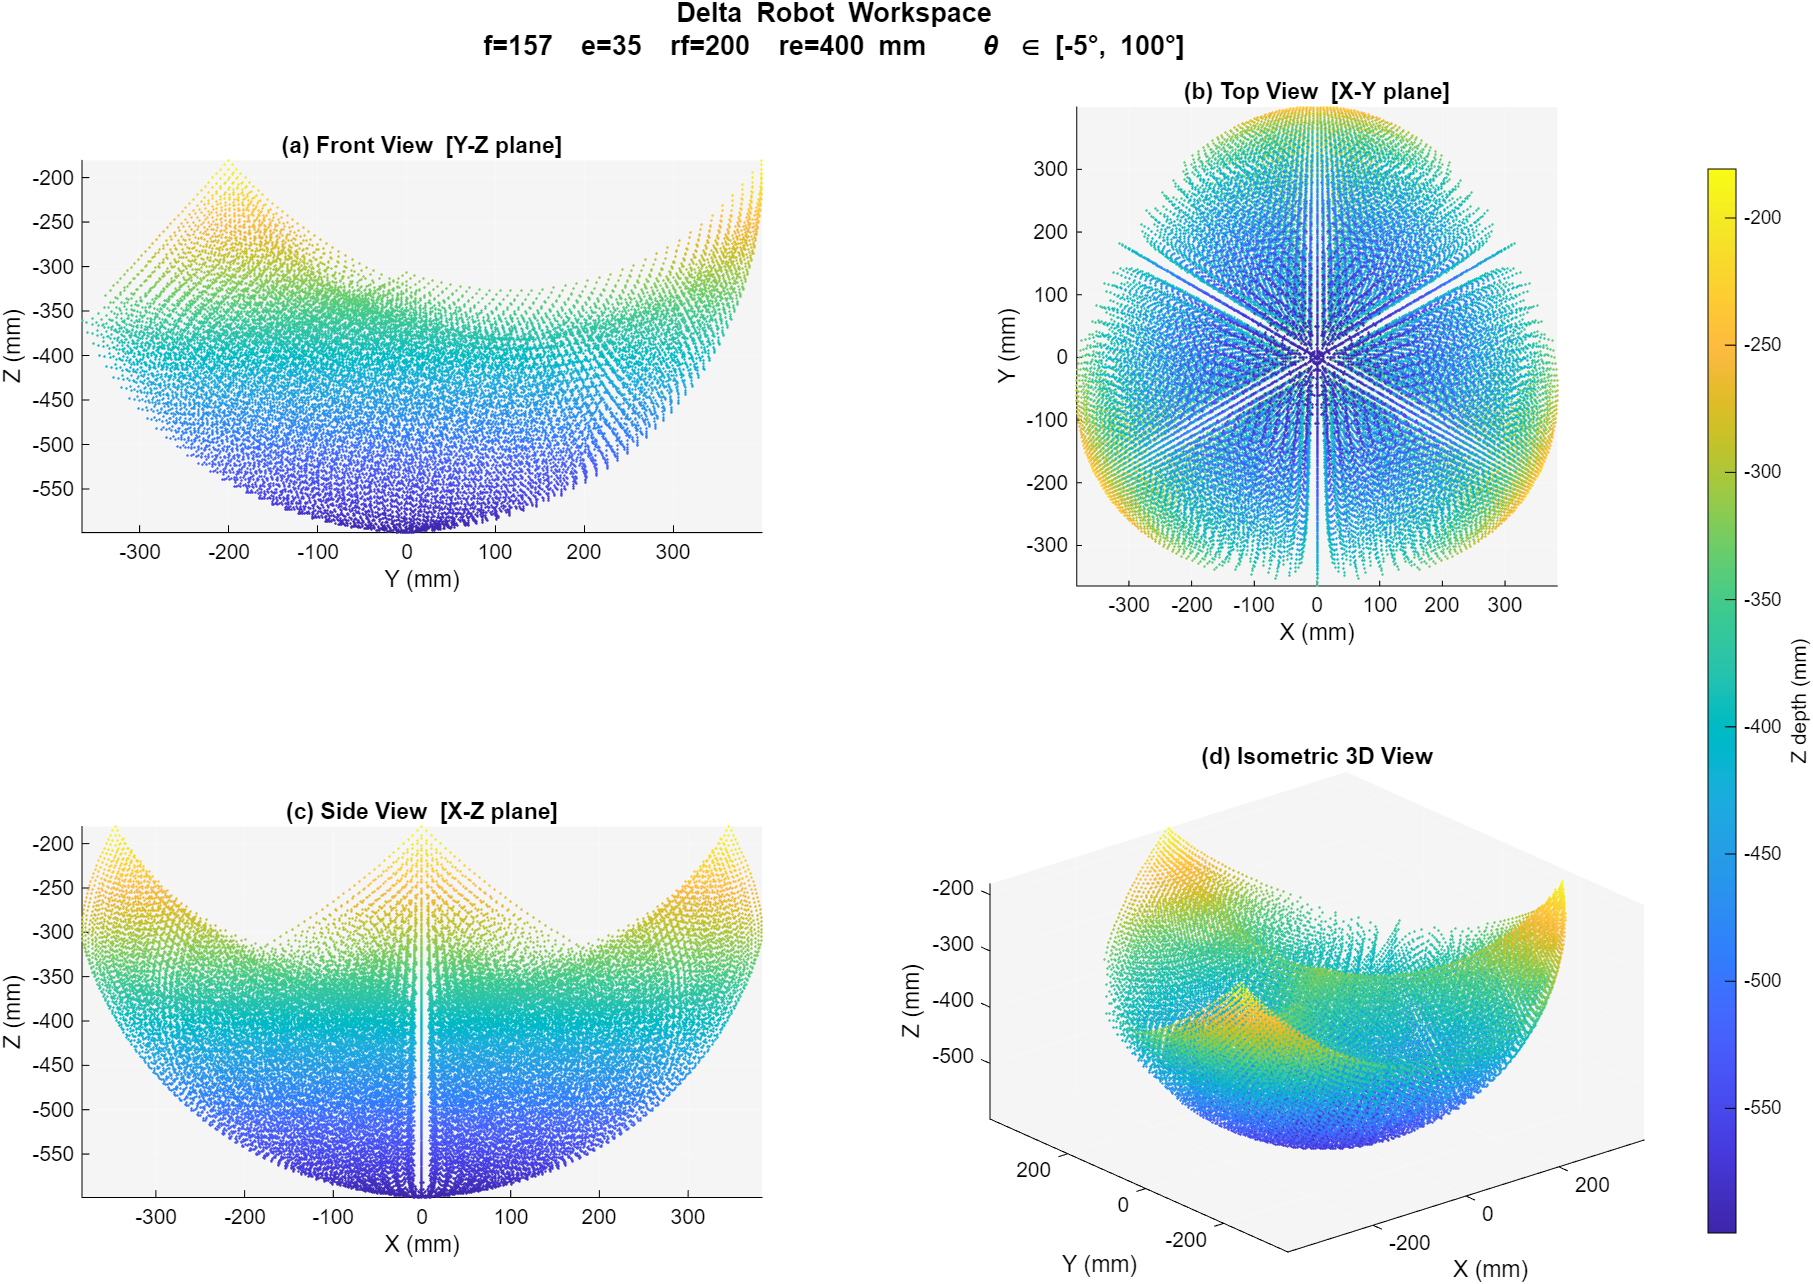
\includegraphics[width=0.9\linewidth]{image/Delta Robot Workspace.png}
    \caption{Full reachable workspace of the Delta robot
             visualised as a 3D point cloud in MATLAB,
             colour-coded by depth $Z$ from the base frame.}
    \label{fig:workspace}
\end{figure}
\par
\hspace{1.27cm}
The full reachable workspace extends considerably beyond the
region that is practically usable for pick-and-place
operations. The upper portions of the workspace (small
negative $Z$ values, yellow-green region in
\textbf{\autoref{fig:actual_workspace}}) correspond to
configurations where the upper arms approach horizontal,
which reduces the effective torque output of the actuators
and brings the forearm parallelograms close to a singular
configuration. The lower boundary is determined by the
maximum extension of the forearms at full vertical reach.
To avoid these mechanical extremes and to constrain the
robot to a region where positioning accuracy and structural
stiffness are reliably maintained, an operational workspace
sub-region was defined as a rectangular box within the
reachable volume, shown by the black rectangle in
\textbf{\autoref{fig:actual_workspace}}.

\begin{figure}[h]
    \centering
    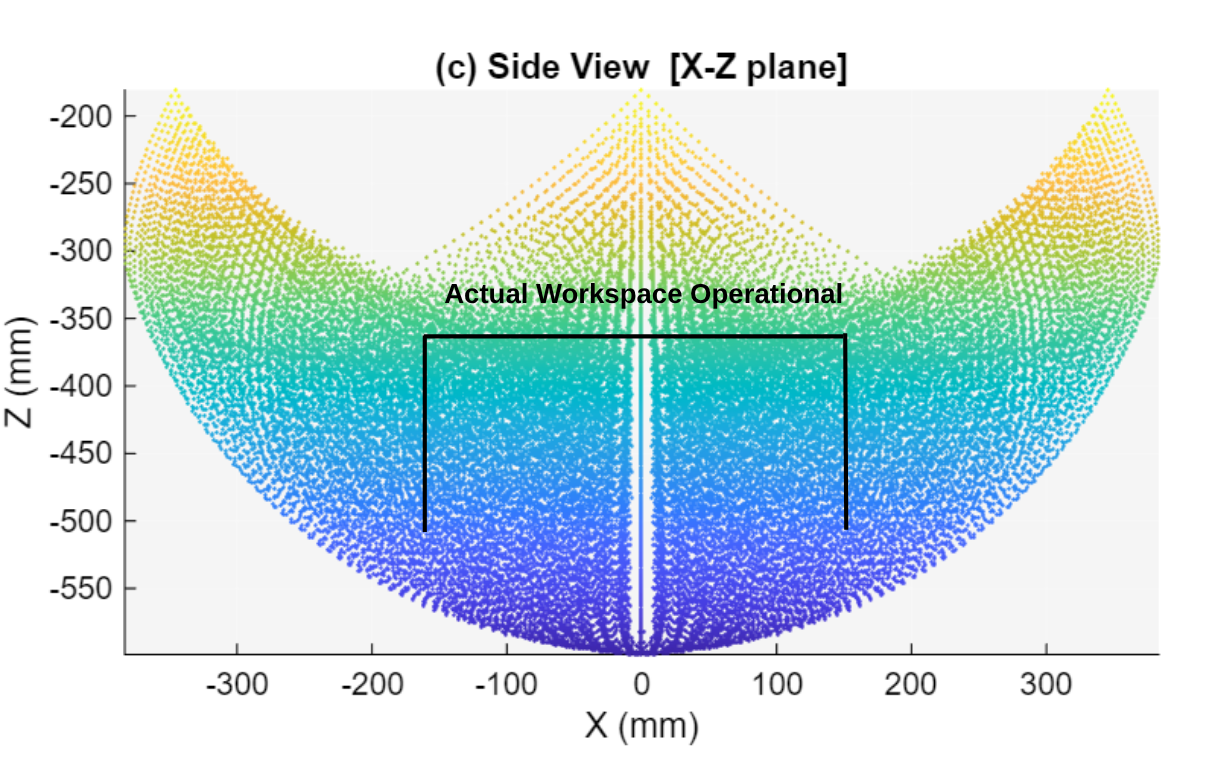
\includegraphics[width=0.7\linewidth]
        {image/Actual worksapce operational.png}
    \caption{Side view (XZ plane) of the full reachable
             workspace with the actual operational workspace
             sub-region indicated by the black rectangle.
             The operational region spans
             $X \in [-150,\, +150]$\,mm and
             $Z \in [-350,\, -500]$\,mm.}
    \label{fig:actual_workspace}
\end{figure}

\par
\hspace{1.27cm}
The physical extent of the operational workspace relative to
the robot structure is shown in
\textbf{\autoref{fig:real_workspace}}. The base frame is
located at the top of the structure, establishing $Z = 0$.
The home position of the end-effector is set at
$(0,\, 0,\, -350)$\,mm, which places the gripper
approximately 350\,mm below the base and serves as the
safe retract position between pick cycles. The conveyor
belt surface lies within the operational depth range of
$Z = -500$\,mm to $Z = -650$\,mm, and the pick-and-place
operations are performed within the horizontal bounds of
$X, Y \in [-150,\, +150]$\,mm. The total vertical travel
from home to the deepest pick position is 300\,mm, and
the total physical height of the robot structure including
the support frame is approximately 650\,mm as annotated in
\textbf{\autoref{fig:real_workspace}}.

\begin{figure}[h]
    \centering
    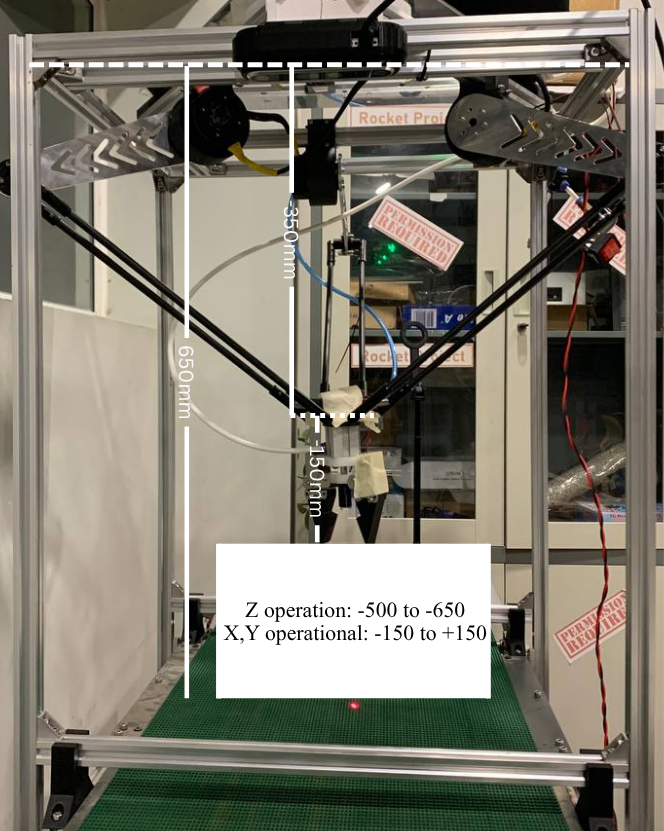
\includegraphics[width=0.525\linewidth]
        {image/real Robot actual operate.png}
    \caption{Physical Delta robot installation showing the
             operational workspace dimensions annotated on
             the real system. The home position is at
             $Z = -350$\,mm below the base frame, and the
             pick depth operates between
             $Z = -500$\,mm and $Z = -650$\,mm. The
             horizontal operational range is
             $X, Y \in [-150,\, +150]$\,mm.}
    \label{fig:real_workspace}
\end{figure}


\par
\hspace{1.27cm}
The operational workspace bounds are enforced in the ROS~2
controller node as hard software limits. Any target
coordinate received from the vision pipeline that falls
outside these bounds is immediately rejected before the
IK solver is invoked, preventing the robot from attempting
to reach a position where accuracy or mechanical safety
cannot be guaranteed. The complete set of software-enforced
workspace parameters is listed in
\textbf{\autoref{tab:workspace}}.
\begin{table}[ht]
    \centering
    \caption{Robot Operational Workspace Parameters.}
    \label{tab:workspace}
    {\small
    \begin{tabular}{lcc}
        \hline
        \textbf{Parameter} & \textbf{Symbol} &
        \textbf{Value} \\
        \hline
        Planar X operational limit  & $X\_LIMIT$
            & $\pm150$\,mm \\
        Planar Y operational limit  & $Y\_LIMIT$
            & $\pm150$\,mm \\
        IK upper ceiling            & $Z\_MAX$
            & $-323$\,mm \\
        Maximum pick depth          & $Z\_MIN$
            & $-560$\,mm \\
        Home position               & $(X_0,Y_0,Z_0)$
            & $(0,\;0,\;-350)$\,mm \\
        Total vertical travel       & $\Delta Z$
            & $210$\,mm \\
        Robot structure height      & $Z\_Belt$
            & $-650$\,mm \\
        \hline
    \end{tabular}}
\end{table}
%============================================================================
%============================================================================
% CONTROL SYSTEM IMPLEMENTATION + VISION PIPELINE
% Institute of Technology of Cambodia
% Delta Robot Vision-Based Control System
% Academic Year: 2025-2026
%============================================================================

\subsection{Control System Implementation}

\subsubsection{System Wiring and Hardware Architecture}
\hspace{1.27cm}
The complete electrical and communication architecture of the
Delta robot system is illustrated in
\textbf{\autoref{fig:wiring_diagram}}. The system is powered
from a 220\,V AC mains supply and is organised into three
distinct subsystems: the Delta robot actuator and CAN bus
subsystem, the conveyor belt drive subsystem, and the
pneumatic gripper subsystem. The host PC running Ubuntu
22.04 and ROS~2 Humble serves as the central computing unit
coordinating all subsystems.

\par
\noindent\textbf{Power Distribution.}\par
\hspace{1.27cm}
A 24\,V regulated DC power supply converts the 220\,V AC
mains input and provides the primary power rail for the
three RobStride RS-00 motor drivers (rated 24\,V). A separate
5\,V rail from the same supply powers the Arduino UNO used for
conveyor belt control. A 24\,V lithium battery pack powers
the DCLAB Smart Driver board that provides the fourth
actuator channel. All power lines are shown as red traces
in \textbf{\autoref{fig:wiring_diagram}}.

\par
\noindent\textbf{CAN Bus Subsystem (Delta Robot Motors).}\par
\hspace{1.27cm}
The three RobStride RS-00 actuators (Motor ID\,1, ID\,2,
and ID\,3) are connected in a daisy-chain CAN bus topology
via CAN\,H and CAN\,L differential signal lines. Each motor
unit integrates a gear stage, the brushless motor body, and
a magnetic encoder within a single compact package. The CAN
bus is interfaced to the host PC through a Makerbase
CANable~V2.0 USB-to-CAN adapter operating on the
\texttt{can0} interface at 1\,Mbit/s. The three motor nodes
drive the three upper arm links (Upper Arm Link~1, 2, and 3)
of the Delta robot respectively. An additional motor is
connected to the DCLAB Smart Driver board via a separate
24\,V power path.

\par
\noindent\textbf{Conveyor Belt Subsystem.}\par
\hspace{1.27cm}
The conveyor belt is driven by a NEMA stepper motor
controlled by a dedicated stepper driver. The stepper driver
receives step and direction pulse signals from an Arduino
UNO, which is powered at 5\,V from the 24\,V supply
auxiliary output. The Arduino UNO communicates with the host
PC via USB serial, allowing the ROS~2 belt prediction node
to read encoder pulses and compute belt velocity. The
complete drive chain from stepper motor through gear and
coil stages to the physical conveyor belt mechanism is
shown in the upper portion of
\textbf{\autoref{fig:wiring_diagram}}.

\par
\noindent\textbf{Pneumatic Gripper Subsystem.}\par
\hspace{1.27cm}
The pneumatic actuation chain begins at an air compressor
that pressurises a portable air container (cylinder).
Compressed air from the container feeds a solenoid valve,
which is controlled by an ON/OFF switch (SW1) signal from
the DCLAB Smart Driver board. When the solenoid is
energised, compressed air is routed to the two-finger
mechanical jaw gripper mounted on the Delta robot
end-effector. The solenoid valve is commanded via the
CAN bus using CAN ID\,4, with command
\texttt{004\#01} to close and \texttt{004\#00} to open,
as described in \autoref{tab:end_effector_components}.

\par
\noindent\textbf{Sensor Interface.}\par
\hspace{1.27cm}
The Intel RealSense D455 camera is connected to the host
PC via a dedicated USB Type-C port. The camera streams RGB
frames and camera intrinsic data directly to the ROS~2
detection node running on the PC. No additional power
supply is required as the camera is bus-powered via USB.

\par
\noindent\textbf{ROS~2 Software Stack.}\par
\hspace{1.27cm}
The ROS~2 software architecture is organised into five
custom packages running on the host PC:
\begin{itemize}
    \item \texttt{delta\_common}: shared kinematic solver,
    system configuration parameters, and error code map.
    \item \texttt{delta\_motor\_controller}: CAN motor
    abstraction layer providing position, velocity, and
    torque command interfaces to the RobStride RS-00
    actuators.
    \item \texttt{delta\_camera\_system}: vision pipeline
    integrating HSV blob detection, YOLO11n inference,
    backprojection, and coordinate transformation.
    \item \texttt{delta\_main\_app}: finite state machine
    controller, belt speed predictor, and visual
    end-effector feedforward correction loop.
    \item \texttt{delta\_can\_driver}: low-level SocketCAN
    interface managing frame encoding, decoding, and
    bus timing for the \texttt{can0} interface.
\end{itemize}
\hspace{1.27cm}
All packages communicate through typed ROS~2 topics,
enabling modular unit testing and independent replacement
of individual subsystems without modifying other packages.

\begin{figure}[h!]
    \centering
    \includegraphics[width=1\linewidth]{image/ros2_architecture.png}
    \caption{Complete system wiring and hardware architecture
             of the Delta robot pick-and-place system,
             showing the 220\,V AC mains input, 24\,V motor
             power supply, CAN bus daisy-chain topology for
             the three RobStride RS-00 actuators, stepper
             motor conveyor drive, pneumatic gripper
             subsystem, and USB interfaces to the host PC.}
    \label{fig:wiring_diagram}
\end{figure}

%--------------------------------------------------------------------
\subsubsection{Task Framework}\label{sec:task_framework}
\hspace{1.27cm}
The pick-and-place task is structured as an 8-state finite
state machine (FSM) illustrated in
\textbf{\autoref{fig:task_framework}}. The FSM runs in a
dedicated background thread to avoid blocking the ROS~2
spin loop. State transitions are triggered by motion
completion (FK error below threshold) or timer events.\par

\begin{figure}[h]
    \centering
    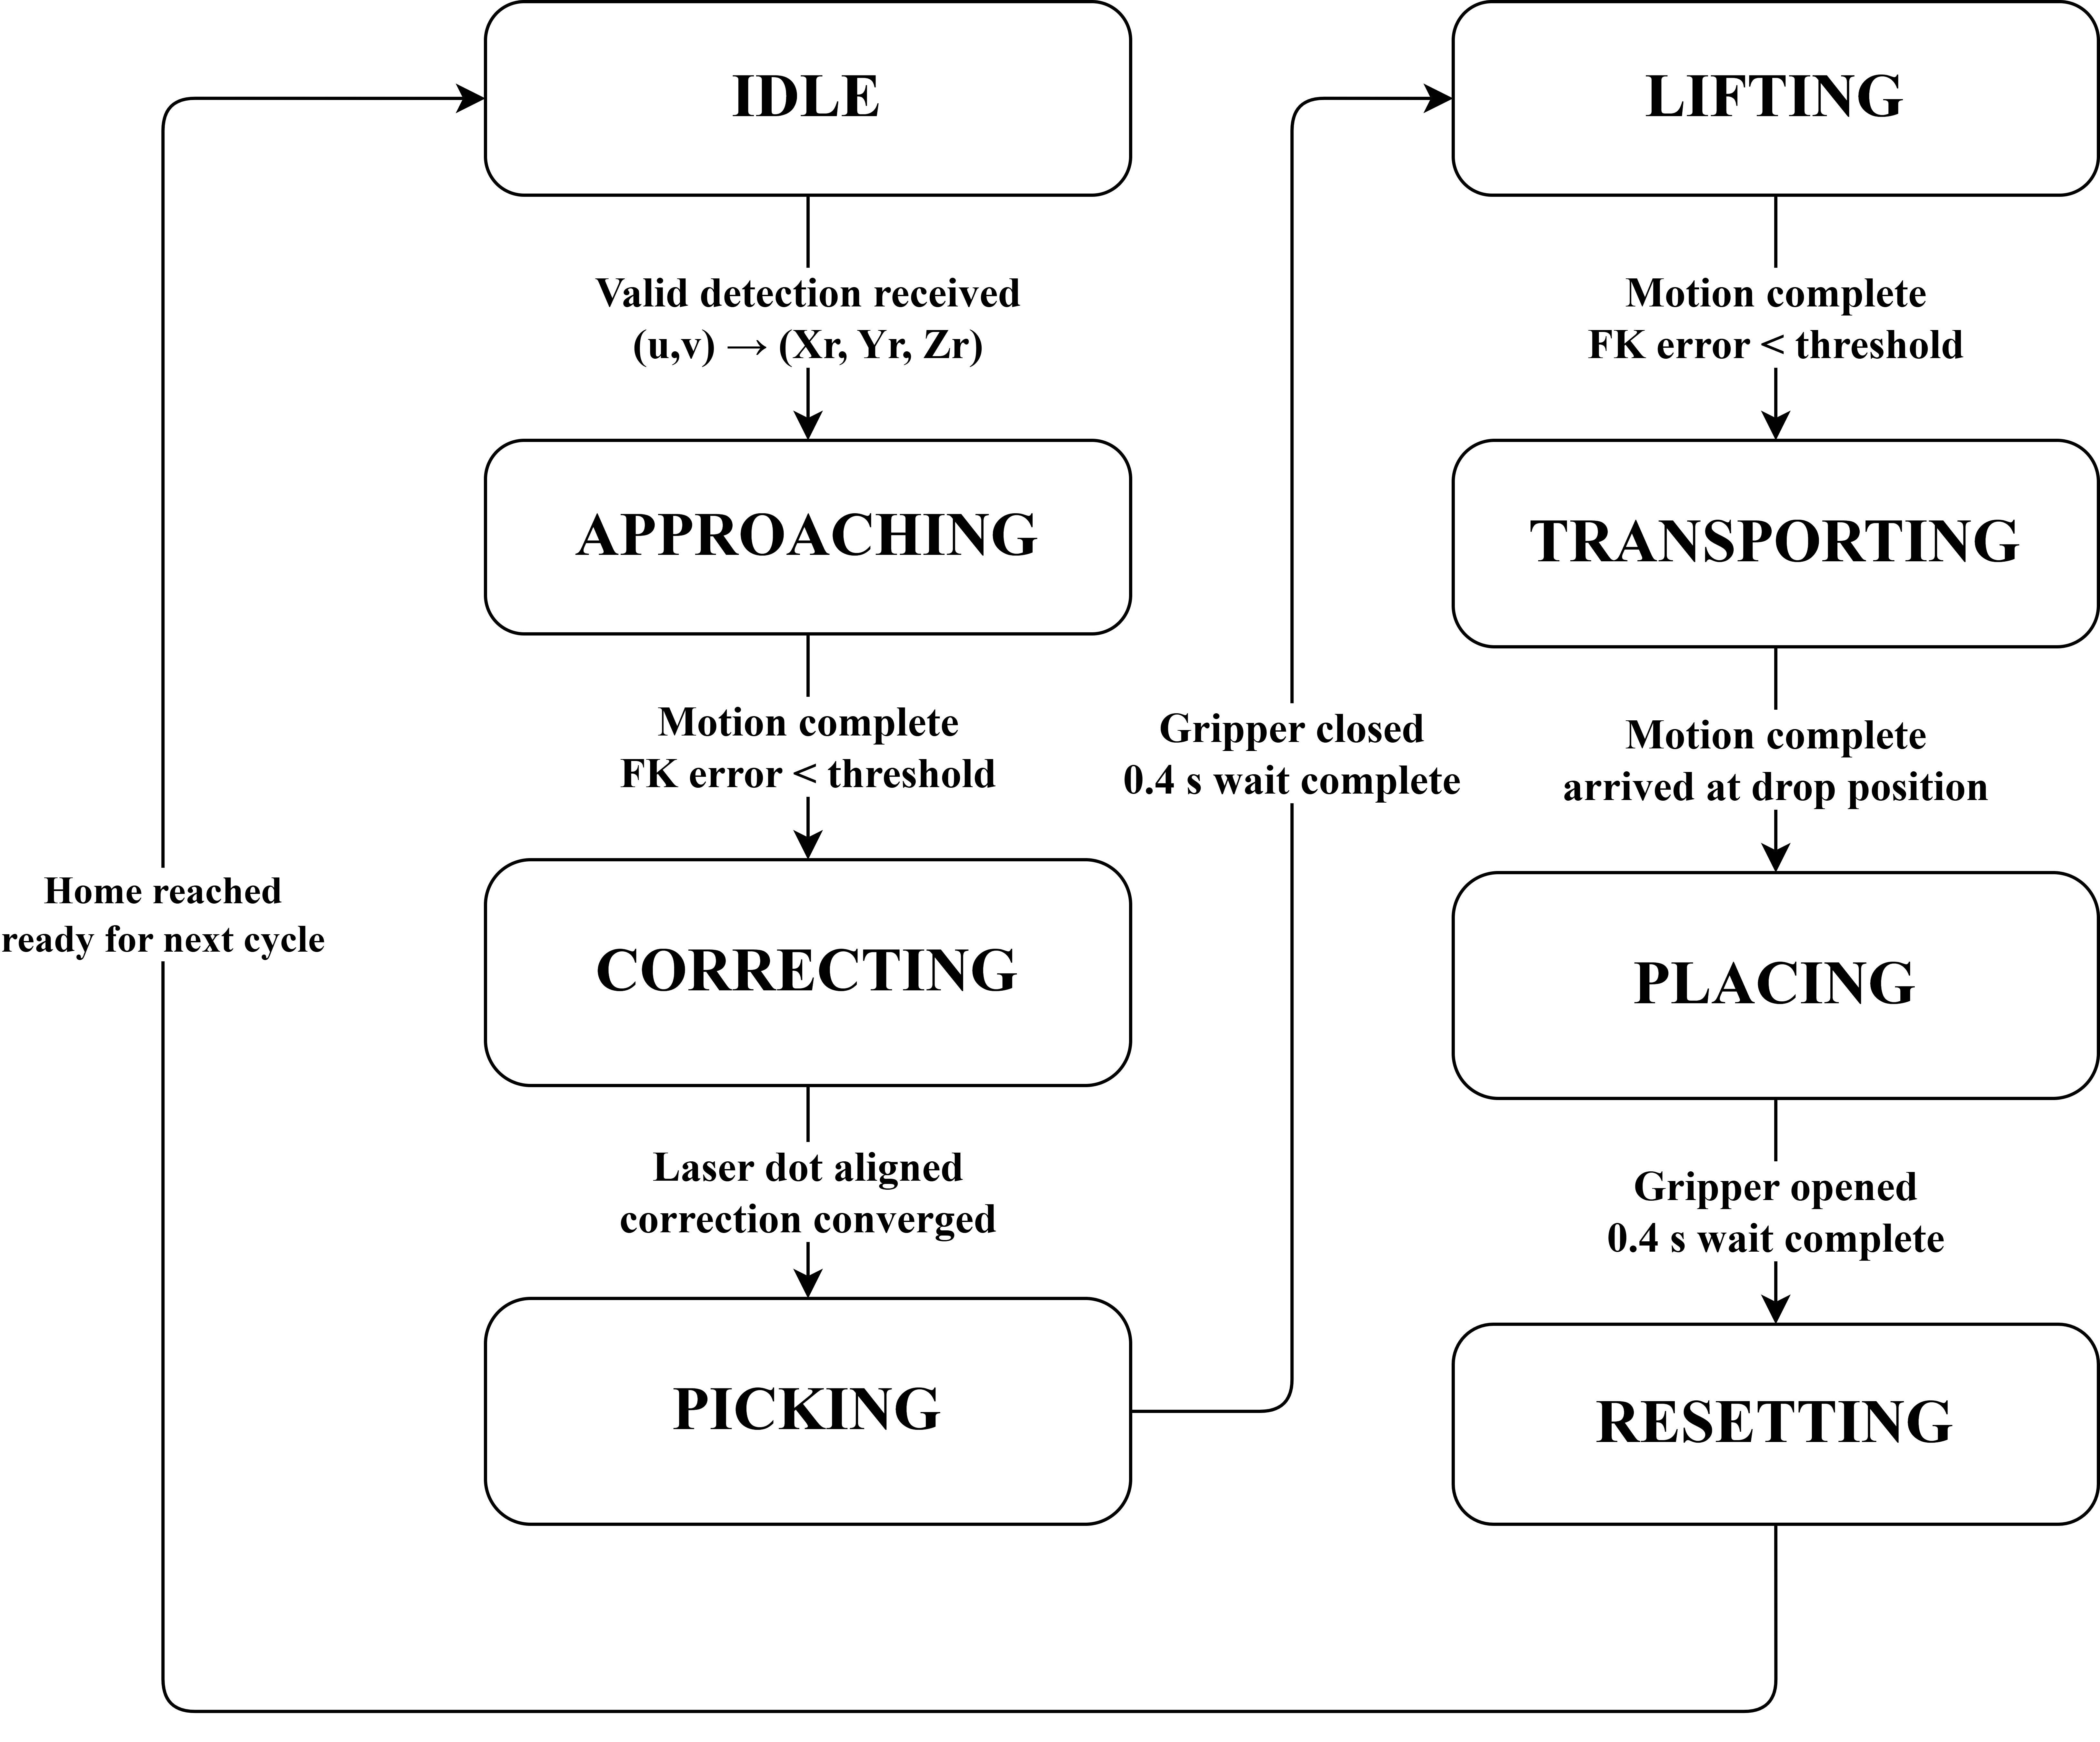
\includegraphics[width=0.45\linewidth]{image/fsm_pick_place.png}
    \caption{Pick-and-Place Finite State Machine (8 States).}
    \label{fig:task_framework}
\end{figure}

\hspace{1.27cm}
The sequence begins in \textbf{IDLE}, where the system
waits for a valid detection from the vision pipeline. Once
a detection is confirmed over \texttt{DETECTION\_CONFIRM\_FRAMES}
consecutive frames, the FSM enters \textbf{APPROACHING},
commanding the end-effector to move horizontally to the
target $(X_r,\, Y_r)$ at approach depth
$z_{\text{approach}} = Z_r$ (no vertical offset, $APPROACH\_Z\_OFFSET = 0$).
During this move, the visual end-effector feedforward correction
loop runs: it detects the laser dot, computes the horizontal offset
between the dot centroid and the object centroid, and issues
iterative position corrections until the X-axis error falls
below \texttt{EE\_CORRECTION\_THRESH\_MM = 3}\,mm. Once
aligned, the FSM transitions to \textbf{PICKING}, descending
to the pick depth $Z_{\text{pick}} = -535$\,mm (platform Z,
corresponding to EE tip at the belt surface), and the
\textbf{GRASPING} state activates the pneumatic gripper,
followed by a 0.4\,s dwell to allow the jaw to fully engage.
The robot then enters \textbf{LIFTING}, ascending to a safe
clearance height of $z_{\text{pick}} + 30$\,mm, before entering
\textbf{TRANSPORTING}, which moves the end-effector horizontally
to the drop position $(150,\, -150,\, -500)$\,mm (platform Z)
at the belt exit. In the \textbf{DROPPING} state the gripper
opens and a 0.4\,s dwell ensures the object is released before
the robot enters \textbf{RESETTING}, returning to the home
position $(0,\, 0,\, -350)$\,mm and transitioning back to IDLE
for the next pick cycle.

%--------------------------------------------------------------------
\subsubsection{Trajectory Planning Algorithm}
\hspace{1.27cm}
Trajectories between Cartesian waypoints are planned using
a triangular velocity profile, which applies when the
travel distance is shorter than the distance required to
reach $v_{\max}$. For the medium motion preset
($v_{\max} = 2000$\,mm/s, $a_{\max} = 5000$\,mm/s$^2$),
the minimum distance required to reach $v_{\max}$ is:

\begin{cequation}
    d_{\text{accel}} = \frac{v_{\max}^2}{2\, a_{\max}}
    = \frac{2000^2}{2 \times 5000} = 400\,\text{mm}.
    \label{eq:daccel}
\end{cequation}

Since all moves within the $\pm$150\,mm workspace are
shorter than $2 \times 400 = 800$\,mm, all trajectories
use the triangular profile, and the travel time for a move
of distance $d$ is:

\begin{cequation}
    t_{\text{move}} = 2\sqrt{\frac{d}{a_{\max}}}.
    \label{eq:tmove}
\end{cequation}

Intermediate Cartesian waypoints are generated by linear
interpolation at time steps of $\Delta t = 0.05$\,s, and
the IK solver is evaluated at each waypoint to produce a
sequence of joint angle commands sent to the motors over
the CAN bus.

%============================================================================
\subsection{Calibration Procedure}\label{sec:calibration}
\hspace{1.27cm}
Before operation, the camera-to-robot coordinate transform
is calibrated to align the projected workspace overlay with
the physical robot workspace. The calibration uses a visual
reference: a white crosshair marker is rendered in the
camera feed at the projected base-frame origin
$(0,\, 0,\, -650)$\,mm. The calibration sequence is as
follows:

\begin{enumerate}
    \item Command the robot to the home position
    $(0,\, 0,\, -350)$\,mm. The red laser dot on the
    end-effector tip indicates the physical robot origin
    projected onto the belt surface in the camera image.

    \item Observe the offset between the crosshair
    position and the laser dot centroid in the live
    camera feed.

    \item Adjust \texttt{CAM\_TX\_MM} in $\pm$10\,mm
    steps until the crosshair aligns horizontally with
    the laser dot.

    \item Adjust \texttt{CAM\_TY\_MM} in $\pm$10\,mm
    steps until the crosshair aligns vertically with
    the laser dot.

    \item Verify calibration by placing a physical object
    at the robot kinematic centre $(0,\, 0)$ and
    confirming that the system reports
    \texttt{BASE = (0, 0, -650)} within $\pm$5\,mm.
\end{enumerate}

\begin{figure}[h]
    \centering
    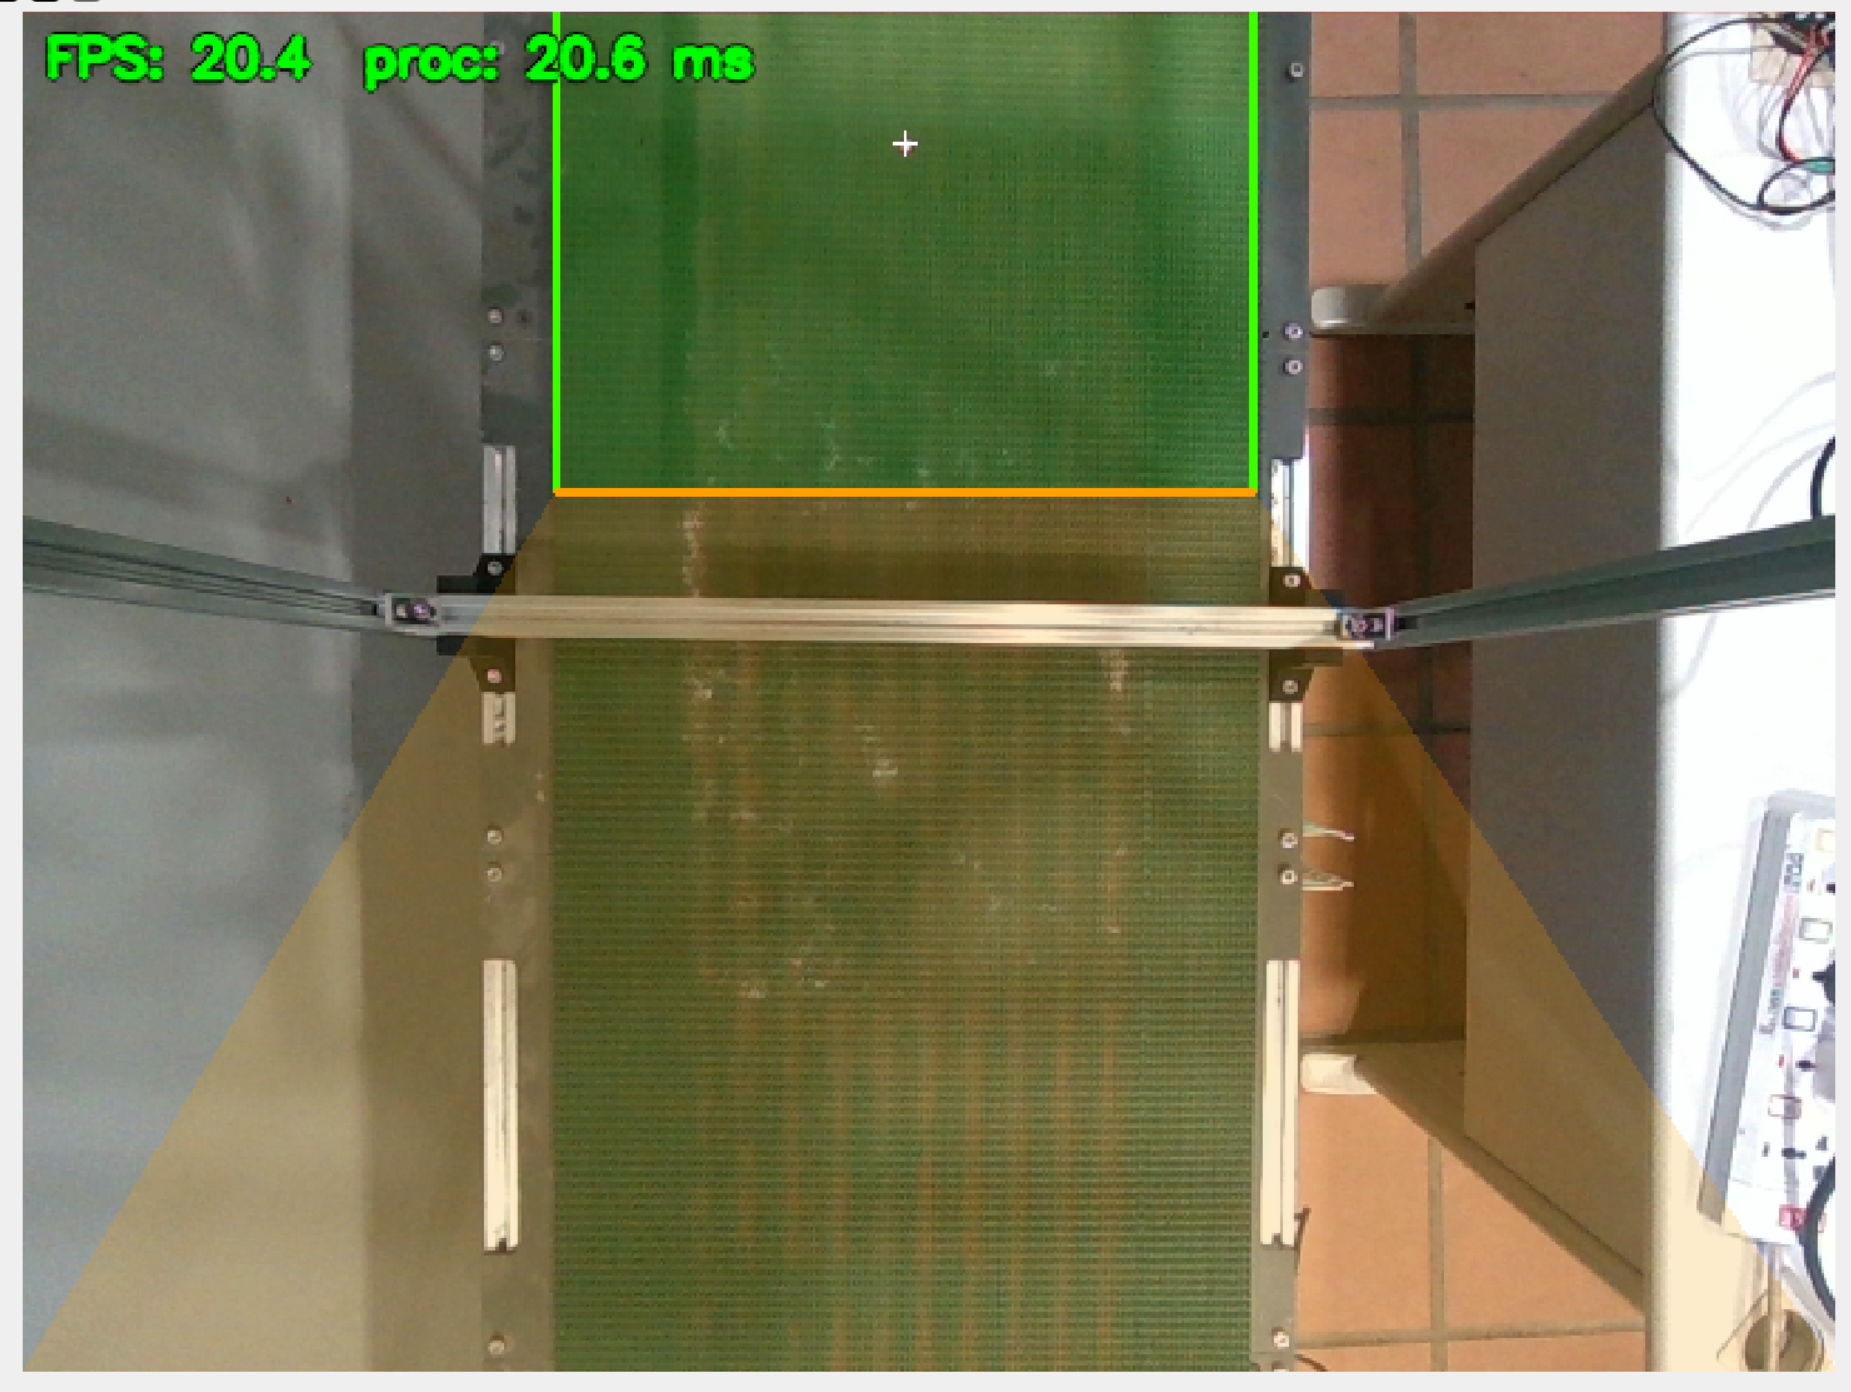
\includegraphics[width=0.5\linewidth]{image/Calibrate WorkSpace.png}
    \caption{Camera calibration: crosshair aligned to the
             end-effector laser dot at the robot kinematic
             origin.}
    \label{fig:calibration_gui}
\end{figure}

\hspace{1.27cm}
The calibrated translation vector for this system is
$\mathbf{t} = [-10.0,\; +235.0,\; -20.0]^{\top}$\,mm.
The parameters \texttt{CAM\_TX\_MM = -10.0}\,mm and
\texttt{CAM\_TY\_MM = 235.0}\,mm are the horizontal X and Y
offsets of the camera optical centre relative to the robot base
frame origin, determined empirically. The parameter
\texttt{CAM\_TZ\_MM = -20.0}\,mm indicates that the camera is
mounted 20\,mm below the robot base frame origin along the
$Z$-axis. The camera-to-belt vertical distance used in the
pinhole backprojection is stored separately as
\texttt{FAKE\_DEPTH\_M = 0.650}\,m (650\,mm), which is the
measured vertical distance from the camera optical centre to
the belt surface at the pick depth.

%============================================================================
\subsection{Vision Pipeline}
\hspace{1.27cm}
The vision pipeline converts raw RGB camera data into robot
base-frame coordinates used by the motion controller. It
consists of four sequential stages as illustrated in
\textbf{\autoref{fig:vision_pipeline}}. The pipeline is
triggered once per incoming colour frame at 15--30\,fps and
produces a validated target position $(X_r,\, Y_r,\, Z_r)$
that is published to the \texttt{/target\_robot\_xyz} topic
for consumption by the IK solver, or discards the frame
silently if any stage fails its validity check.

\begin{figure}[h]
    \centering
    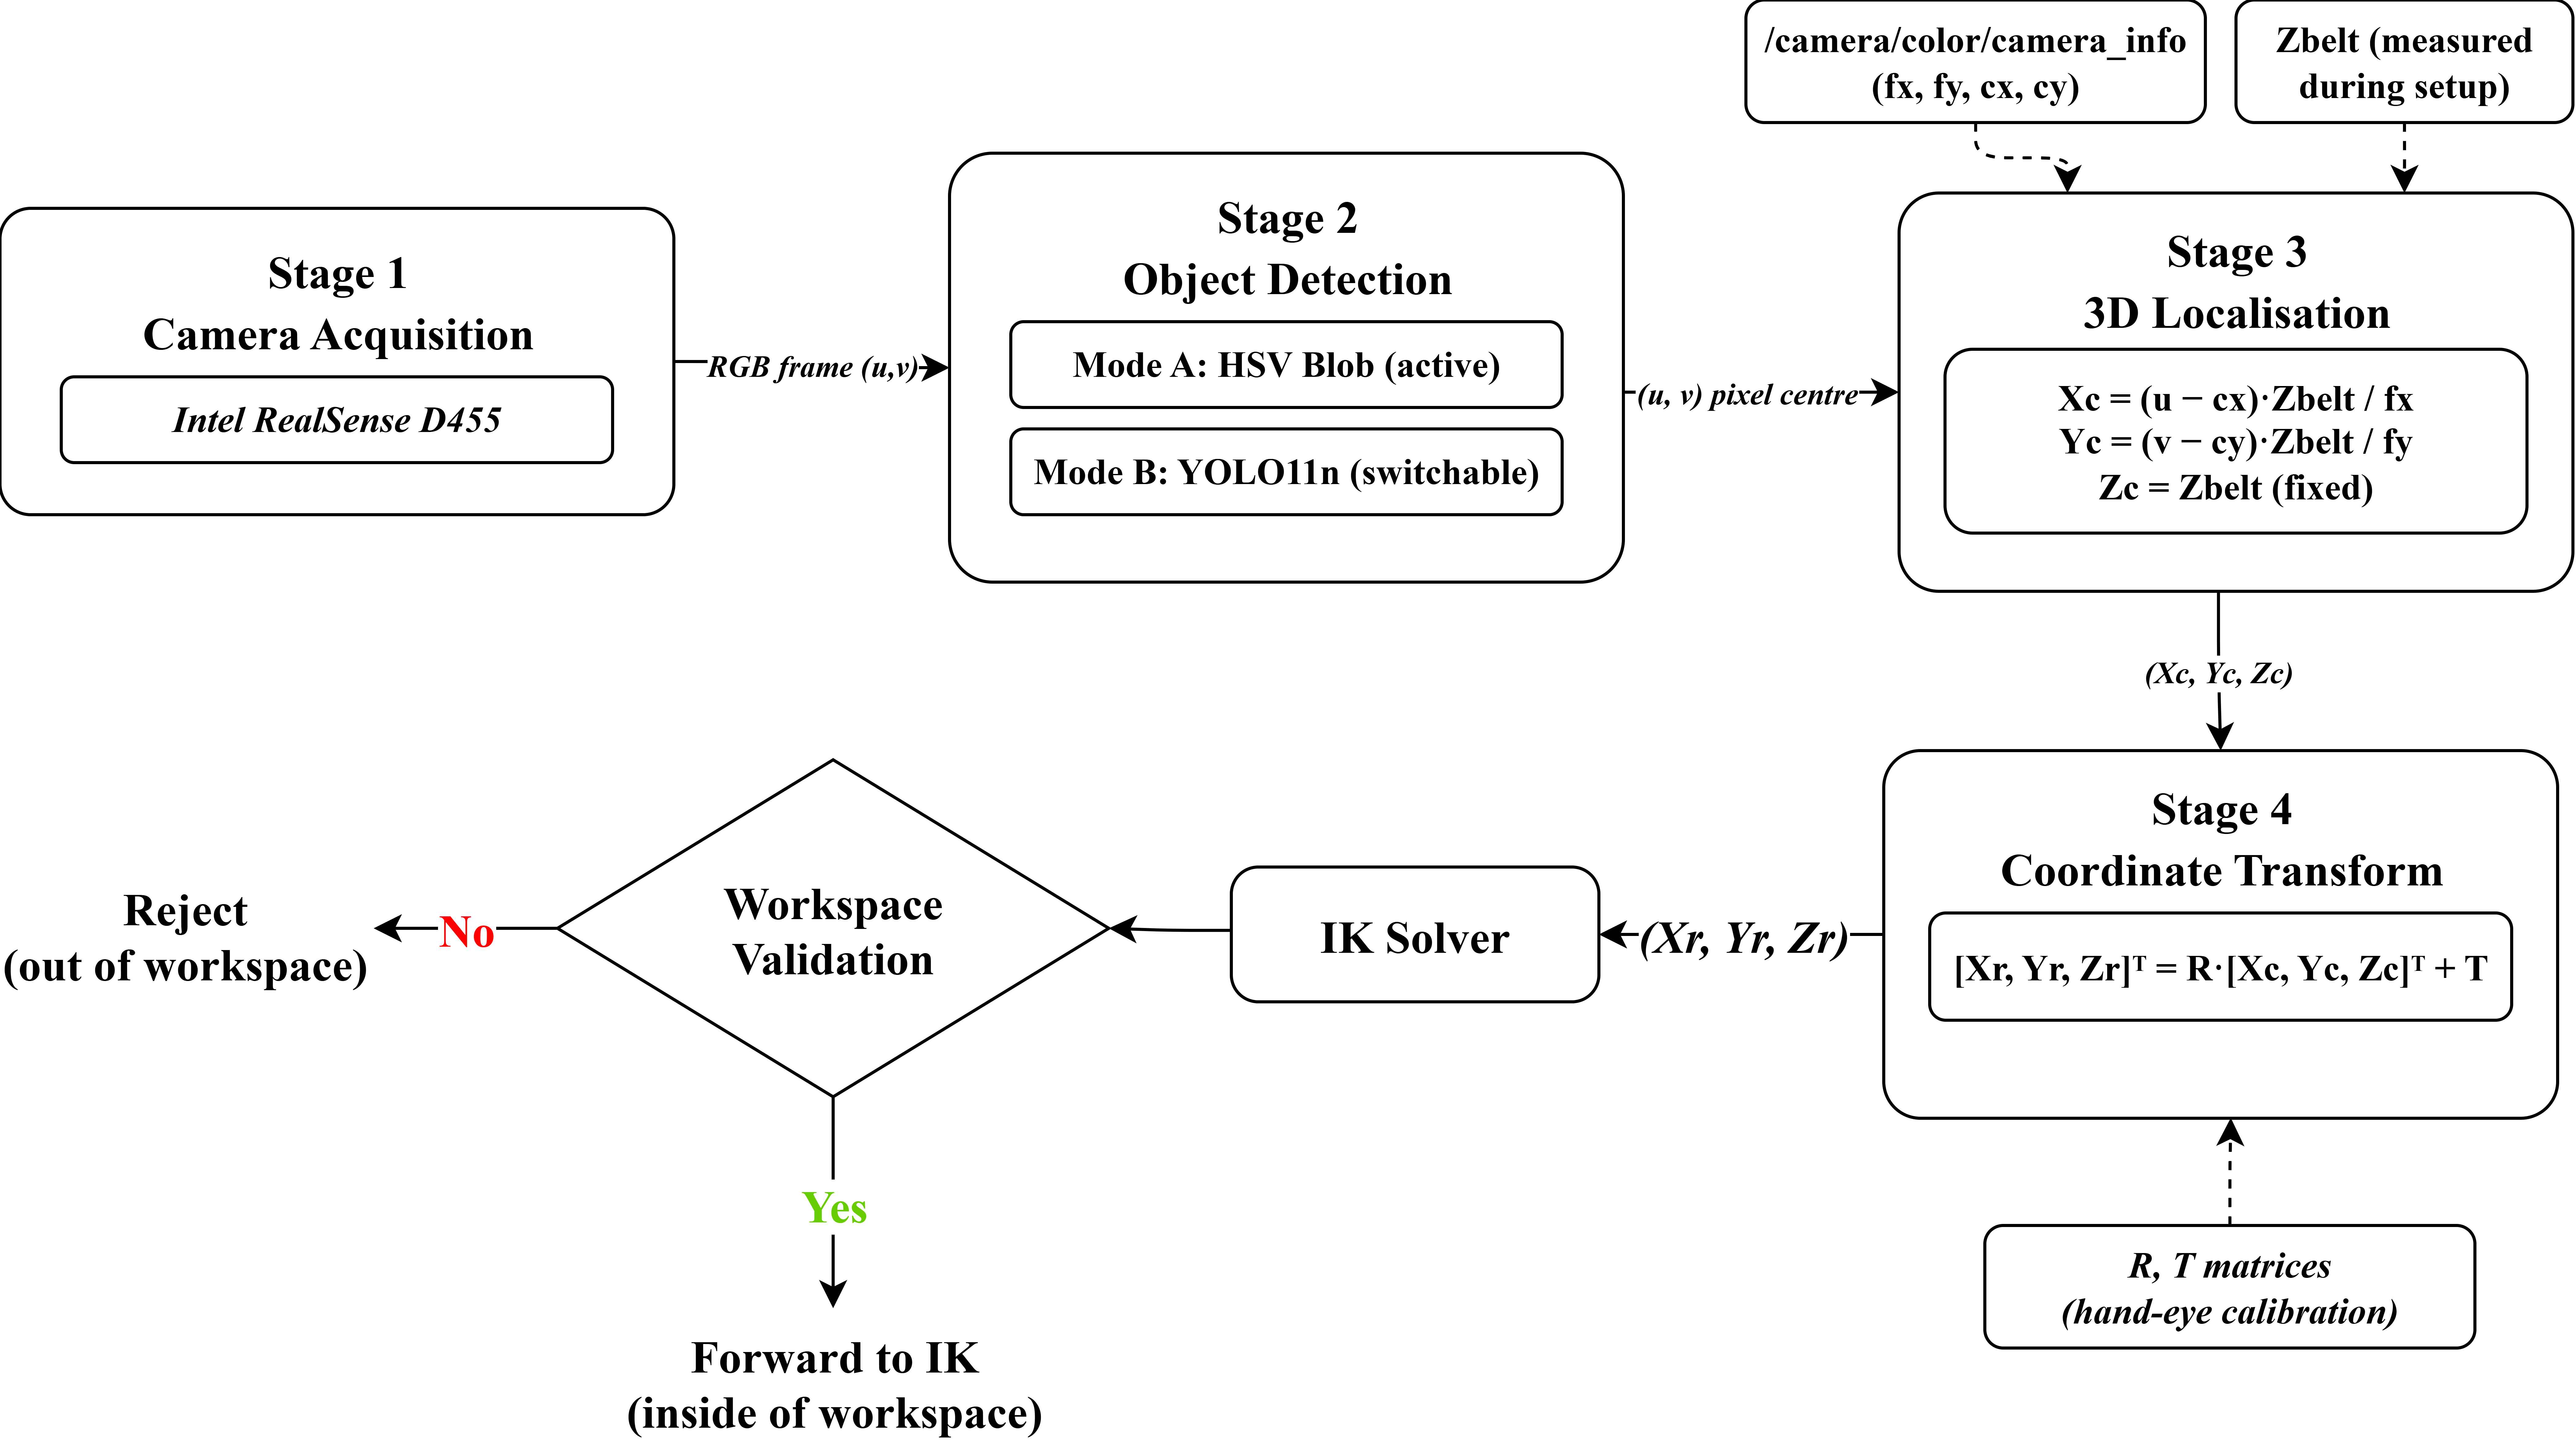
\includegraphics[width=0.72\linewidth]{image/vision_pipeline.png}
    \caption{Vision-to-Motion Pipeline: Stage Architecture.}
    \label{fig:vision_pipeline}
\end{figure}

%--------------------------------------------------------------------
\subsubsection{Camera Hardware and ROS~2 Topics}
\hspace{1.27cm}
The Intel RealSense D455 camera is mounted overhead,
directed vertically downward at the workspace. Although the
D455 is capable of stereo depth sensing with a 95\,mm
baseline and structured infrared illumination, only its RGB
colour stream is used in this system. The conveyor belt
surface lies at a fixed and known elevation of approximately
$Z_{\text{belt}} = -650$\,mm below the robot base frame (EE-tip
coordinate; platform Z at pick $= -535$\,mm),
so per-pixel depth measurement is unnecessary: the $Z$
coordinate of every pick target is constant by
construction, eliminating the need to process the depth
stream entirely and reducing pipeline latency. The camera
provides the following ROS~2 topics consumed by the
detection node:

\begin{itemize}
    \item \texttt{/camera/camera/color/image\_raw}:
    RGB image at $640 \times 480$\,px, 30\,fps,
    published as \texttt{sensor\_msgs/Image} in BGR8
    encoding.
    \item \texttt{/camera/camera/color/camera\_info}:
    camera intrinsic matrix $\mathbf{K}$ containing
    focal lengths $(f_x,\, f_y)$ and principal-point
    coordinates $(c_x,\, c_y)$, read once at node
    startup and cached for the session.
\end{itemize}

\hspace{1.27cm}
Reading the intrinsic parameters live from the
\texttt{camera\_info} topic rather than a static
configuration file ensures that the correct calibration
is used regardless of any change in camera resolution or
mounting position, since the RealSense driver recomputes
and republishes intrinsics appropriate to the active
stream profile on every startup.

%--------------------------------------------------------------------
\subsubsection{Object Detection}
\hspace{1.27cm}
Object detection is performed by a configurable detection
node that supports two interchangeable modes, selected
via the \texttt{DETECTION\_MODE} parameter in
\texttt{config.py}. Both modes produce the same output
interface: a single pixel coordinate $(u,\, v)$
representing the centroid of the detected target object.
The live camera feed with all overlays active is shown
in \textbf{\autoref{fig:detection_feed}}, where the
system is running at 30\,fps with a processing latency
of 5.3\,ms per frame.
\begin{figure}[h]
    \centering
    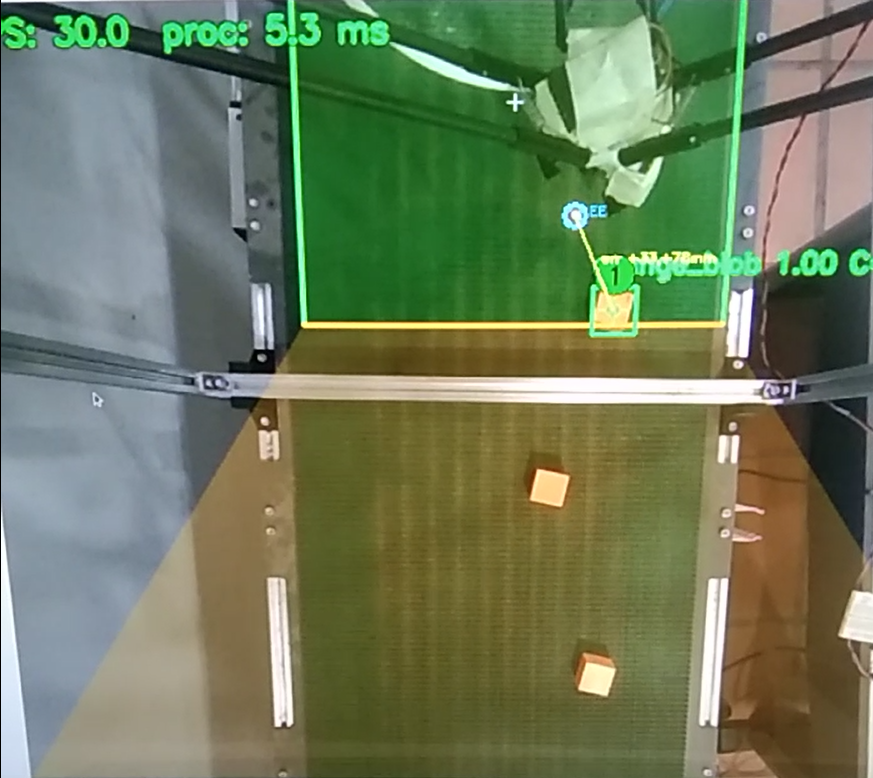
\includegraphics[width=0.55\linewidth]{image/EE and obj detection.png}
    \caption{Live camera feed from the RealSense D455
             during active pick-and-place operation at
             30\,fps (proc: 5.3\,ms). The green rectangle
             marks the operational workspace boundary. The
             detected orange cube is enclosed by a green
             bounding box labelled \texttt{orange\_blob}
             with confidence 1.00. The cyan \texttt{EE}
             circle indicates the projected end-effector
             laser dot position, connected by a yellow
             offset line to the object centroid showing
             the active EE correction residual. The yellow
             horizontal line is the belt prediction
             overlay. Two additional orange cubes are
             visible on the belt outside the workspace
             boundary and are correctly ignored by the
             detection node.}
    \label{fig:detection_feed}
\end{figure}


\par
\hspace{1.27cm}
\textbf{orange\_blob mode (active).} HSV colour-space
filtering detects the target object by applying a
dual-range hue threshold tuned to the orange target
colour. The algorithm converts each incoming BGR frame
to HSV, applies the threshold masks, and identifies the
largest valid contour in the resulting binary image. The
centroid of this contour is computed using image moments
and returned as the pixel coordinate $(u,\, v)$. As
visible in \textbf{\autoref{fig:detection_feed}}, the
detected orange cube is enclosed by a green bounding box
and labelled \texttt{orange\_blob} with a detection
confidence of 1.00, confirming reliable detection under
the controlled green-screen background of the workspace.
This mode achieves 30\,fps on CPU with a processing time
of 5.3\,ms per frame and zero model loading overhead,
providing deterministic, low-latency detection under
controlled lighting conditions.

\par
\hspace{1.27cm}
\textbf{yolo mode (implemented, switchable).}
YOLO11n (\texttt{yolo11n.pt}, Ultralytics) provides
deep learning-based object detection. The bounding box
centre of the highest-confidence detection above the
configured score threshold is used as the pixel
coordinate $(u,\, v)$. This mode requires the trained
weights file to be present and a configured target class
index in \texttt{config.py}. It is integrated and ready
for activation but was not used for primary system
validation due to its higher CPU inference latency
compared to the HSV mode.

\par
\hspace{1.27cm}
The camera feed in \textbf{\autoref{fig:detection_feed}}
also shows three additional overlays generated by the
detection node. The \textbf{green rectangle} defines the
operational workspace boundary within the camera field of
view: only objects whose detected centroids fall inside
this boundary are forwarded to the coordinate transform
stage. The \textbf{yellow horizontal line} is the belt
prediction overlay, representing the estimated conveyor
belt position at the future pick instant computed by the
belt prediction node. The \textbf{cyan circle} labelled
\texttt{EE} marks the current projected position of the
end-effector laser dot on the belt surface as tracked by
the visual correction loop, and the yellow connecting line
drawn from the \texttt{EE} marker to the detected object
centroid represents the residual offset $(\Delta u,\,
\Delta v)$ that the EE feedforward correction loop is
actively minimising. Frames for which no valid detection
is returned, either because no object is present within
the workspace boundary, the detected contour area falls
below the minimum size threshold, or the YOLO confidence
is below the minimum score, are discarded without
publishing any target, and the pipeline waits for the
next frame.


%--------------------------------------------------------------------
\subsubsection{Pixel-to-Camera-Frame Conversion}
\hspace{1.27cm}
Given the detected pixel coordinate $(u,\, v)$ and the
camera intrinsic parameters $(f_x,\, f_y,\, c_x,\, c_y)$
read from the \texttt{camera\_info} topic, the
corresponding 3D point in the camera coordinate frame is
computed using the fixed-height backprojection derived
from the pinhole camera model \autocite{hartley-2004}:

\begin{cequation}
    X_c = \frac{(u - c_x)}{f_x} \cdot Z_{\text{fixed}},
    \qquad
    Y_c = \frac{(v - c_y)}{f_y} \cdot Z_{\text{fixed}},
    \qquad
    Z_c = Z_{\text{fixed}},
    \label{eq:pixel_to_cam}
\end{cequation}

where $Z_{\text{fixed}}$ is stored as the configuration
parameter \texttt{FAKE\_DEPTH\_M = 0.650\,m} (650\,mm) and
represents the measured vertical distance from the camera
optical centre to the belt surface. This conversion is valid
because all pick targets rest on the conveyor belt at a
constant known depth below the camera, so the fixed-$Z$
assumption holds for every frame without exception. No depth
image or per-frame depth measurement is required.

%--------------------------------------------------------------------
\subsubsection{Camera-to-Robot Frame Transform}\label{sec:coordinate_transform}
\hspace{1.27cm}
The camera-frame 3D point
$\mathbf{p}_c = [X_c,\, Y_c,\, Z_c]^{\top}$ is mapped to
the robot base frame through the calibrated rigid-body
transformation \autocite{tsai-lenz-1989}:

\begin{cequation}
    \mathbf{p}_{\text{base}}
    = \mathbf{R}\, \mathbf{p}_c + \mathbf{t},
    \label{eq:transform_pipeline}
\end{cequation}

where the rotation matrix $\mathbf{R}$ encodes the axis
orientation and sign conventions between the two frames,
and the translation vector $\mathbf{t}$ encodes the
physical mounting offset of the camera optical centre
relative to the robot base-frame origin. The calibrated
values used in this system are:

\begin{cequation}
    \mathbf{R} =
    \begin{bmatrix}
        -1 & 0 &  0 \\
         0 & 1 &  0 \\
         0 & 0 & -1
    \end{bmatrix},
    \qquad
    \mathbf{t} =
    \begin{bmatrix}
        -10.0 \\ +235.0 \\ -20.0
    \end{bmatrix} \text{mm}.
    \label{eq:R_and_t}
\end{cequation}

\hspace{1.27cm}
The $-1$ entries in $\mathbf{R}$ reflect the axis sign
inversions required to align the camera coordinate frame
(where the $X$-axis points right and $Z$ points into the
scene) with the robot base frame (where $X$ points in the
robot positive direction and $Z$ points downward from the
base). The diagonal structure confirms that no axis swap
is present: each robot-frame axis corresponds to exactly
one camera-frame axis with a possible sign flip. The
translation offsets $t_x = -10.0$\,mm,
$t_y = +235.0$\,mm, and $t_z = -20.0$\,mm were
determined during the empirical calibration procedure
described in \autoref{sec:calibration} by placing a
reference object at the robot kinematic centre and
iteratively adjusting the offsets until the reported
base-frame coordinates matched the known physical
position.

\par
\hspace{1.27cm}
The resulting robot base-frame coordinates
$(X_r,\, Y_r)$ from \autoref{eq:transform_pipeline} are
paired with the fixed pick height $Z_r = -535$\,mm (platform Z,
corresponding to EE tip at the belt surface) to
form the complete 3D target position
$(X_r,\, Y_r,\, -535)$\,mm, which is then subject to
workspace validation before being passed to the inverse
kinematics solver. The coordinate transform geometry and
the relationship between the camera and robot frames are
illustrated in \textbf{\autoref{fig:camera_transform}}.

\begin{figure}[h]
    \centering
    \includegraphics[width=0.50\linewidth]{image/coordernationTransform.png}
    \caption{Camera-to-Robot Coordinate Transform Diagram
             showing the axis relationships between the
             RealSense D455 camera frame and the Delta robot
             base frame, with the calibrated rotation matrix
             $\mathbf{R}$ and translation $\mathbf{t}$
             annotated.}
    \label{fig:camera_transform}
\end{figure}

%--------------------------------------------------------------------
\subsubsection{Workspace Validation}
\hspace{1.27cm}
Before the target coordinate is published to the
controller, the robot-frame position
$(X_r,\, Y_r,\, Z_r)$ is checked against the operational
workspace bounds defined in \autoref{tab:workspace}:

\begin{itemize}
    \item $|X_r| \leq 150$\,mm
    \item $|Y_r| \leq 150$\,mm
    \item $Z_{\min} \leq Z_r \leq Z_{\max}$
\end{itemize}

\hspace{1.27cm}
Any target position that violates any of these constraints
is discarded and a warning is logged to the ROS~2 console.
Only positions that pass all three checks are published on
the \texttt{/target\_robot\_xyz} topic as a
\texttt{geometry\_msgs/Point} message and consumed by the
FSM controller node as the IK input target. This safety
layer prevents the IK solver from being invoked on
geometrically unreachable positions and protects the
mechanical structure from commands that would drive the
arms into a singular or over-extended configuration.

%============================================================================
% END OF SECTION
%============================================================================
%============================================================================
% END OF VISION PIPELINE SECTION
%============================================================================

\subsection{ROS\,2 System Architecture}
\hspace{1.27cm}
The complete system is implemented as five ROS\,2 packages communicating via topics and services, as shown in \textbf{\autoref{fig:ros2_architecture}}.

\par
\begin{figure}[h]
    \centering
    \includegraphics[width=1.0\linewidth]{image/ros2_architecture_wiring-ROS 2 System Architecture.png}
    \caption{ROS\,2 System Architecture Node and Topic Graph.}
    \label{fig:ros2_architecture}
\end{figure}


